\documentclass{wrcecapstone}

% Known issues:
% Does not incorporate Dr Allison Webster Giddings comments from end of EW401
% No tool for scaling range endurance payload
% No consideration of tradeoffs of sensor resolution, speed, altitude, range
% Machine vision afterthought, no serious use of CNNs to detect plants, not even hello world
% No refs in post Covid text at all
% Operating procedures did not look at Duke Marine Lab UAS procedures
% Did not simulate Matrice ever

\usepackage[separate-uncertainty=true,multi-part-units=single]{siunitx}
\DeclareSIUnit{\year}{y}
\DeclareSIUnit{\inch}{in}
\DeclareSIUnit{\foot}{ft}
\DeclareSIUnit{\poundforce}{lbf}
\DeclareSIUnit{\pound}{lb}
\DeclareSIUnit{\frame}{frame}
\DeclareSIUnit{\mph}{mph}
\DeclareSIUnit{\mile}{mi}
\DeclareSIUnit{\nauticalmile}{nm}
\DeclareSIUnit{\fahrenheit}{F}
\usepackage{graphicx} % covered in WRCE capstone
\usepackage[noadjust]{cite}
\bibliographystyle{IEEEtran}
\usepackage[plain]{fancyref}
\usepackage{amsmath,amsfonts,amssymb}
\usepackage{booktabs}
\usepackage{listings}
\lstset{%
  basicstyle=\ttfamily,
  columns=fullflexible,
  showstringspaces=false}
\lstdefinestyle{mbedC}{
	language=C,
	basicstyle=\ttfamily,
	keywordstyle=\color{blue}\ttfamily,
	stringstyle=\color{magenta}\ttfamily,
	commentstyle=\color{green}\ttfamily,
	directivestyle=\color{red}\ttfamily,
 	morecomment=[l][\color{red}]{\#},
	columns=fullflexible,
	showstringspaces=false,
%	frame=single
}
\lstdefinestyle{usnaMatlab}{
	basicstyle=\ttfamily,
	keywordstyle=\color{blue}\ttfamily,
	stringstyle=\color{magenta}\ttfamily,
	commentstyle=\color{green}\ttfamily,
 	morecomment=[l][\color{red}]{\#},
	columns=fullflexible,
	showstringspaces=false,
	language=Matlab
%	%backgroundcolor=\color{lightgray},
%	frame=single
}
%\usepackage[dvipsnames,svgnames]{xcolor} % partially covered in WRCE capstone
%\usepackage{hyperref} % covered in WRCE capstone
%\hypersetup{%
%  colorlinks=true,
%  linkcolor=violet,
%  urlcolor=blue,
%  citecolor=blue}
%\usepackage{fullpage}
\usepackage{svg}
%\usepackage{svg-extract}
\usepackage[inputamerican,english,cleanlook]{isodate}

\newcommand{\Matlab}{Matlab}
\newcommand{\Dudleyanesiotica}{\emph{Dudleya nesiotica}}
\newcommand{\Dnesiotica}{\emph{D.~nesoitica}}
\newcommand{\Dudleya}{\emph{Dudleya}}
\newcommand{\Malvaassurgentiflora}{\emph{Malva assurgentiflora}}
\newcommand{\Massurgentiflora}{\emph{M.~assurgentiflora}}
\newcommand{\Malva}{\emph{Malva}}

\title{Biomechanics Secure Terrestrial {\nobreak Ecological} Vegetation Extractor (STEVE)}
\student{Midshipman~1/C~Reina~Carroll, Midshipman~1/C~Jacob~Kang, Midshipman~1/C~Ji~Lim, Midshipman ~1/C~Bryan~Phan, and Midshipman~2/C~Levi~Hofland}
\author{Reina~Carroll, Jacob~Kang, Ji~Lim, Bryan~Phan, and Levi~Hofland\thanks{}}
%\contactinfo{bryanphan168@gmail.com, jmkang1998@gmail.com, jlim225@gmail.com, reinscarroll@gmail.com, samsgaffer@gmail.com}
\advisor{Assistant Professor D.~Evangelista}
\departmentchair{Professor B.~Bishop}
\date{\today}

\begin{document}
\maketitlepage
\cleardoublepage
\tableofcontents
\listoffigures
\listoftables

% first page
\clearpage
\maketitle


\begin{abstract}
Environmental and ecological research are often constrained by the accessibility of desired areas to obtain samples. In botanical fields of study, there has been an increased use of unmanned aerial systems (UAS) for surveying and identifying plants growing in these inaccessible areas. However, there is minimal research in UAS plant collection. We will discuss the development of a UAS attached with an extraction device by considering the system’s operating time, payload capacity, reliability of extraction, and resistance to the forces of nature. Our design is focused on development in radio/control, software engineering, electrically powered mechanical systems, cutting methods for plants, 3D printing, and UAS flight operations. The location and geography of the operation environment motivates the designs of the project. We will present concept designs and initial prototyping for the operation mission: (1) to survey a specified area for expert botanist to identify desired plants; (2) to reach to the desired plant in the inaccessible location; and (3) to extract, secure, and recover a sample of the plant from the inaccessible location. We will also discuss the logistics and qualifications required for the team and plans for the operation to support the botanist mission. The UAS design we develop is tailored towards the need of botanists and their research, and we envision further develop in the capabilities of the UAS to support potential missions in industry or the military.
\end{abstract}
\footnotetext{Bryan Phan, Jacob Kang, and Ji Lim are with the Department of Weapons, Robotics, and Control Engineering at the United States Naval Academy. Reina Carroll and Levi Hofland are with the Department of Mechanical Engineering. Addresses for correspondence: \emph{bryanphan168@gmail.com}, \emph{jmkang1998@gmail.com}, \emph{jlim225@gmail.com}, \emph{reinscarroll@gmail.com}, \emph{samsgaffer@gmail.com}}

\section{Introduction}

\subsection{Customer interview}
Dr. Matt Guilliams, a plant systematist and curator of the Santa Barbara Botanical Garden's Clifton Smith Herbarium, studies the flora of California including floristics, biodiversity description, inferring evolutionary patterns, and genetic conservation of rare plants. He is currently researching the endemic species of flora on the Channel Islands. Endemic refers to species of flora or fauna that only exists in specific areas of the world. Dr. Matt Guilliams wants to identify and collect samples of understudied species of flora on the Channel Islands off the coast of Santa Barbara because he seeks to protect the endemic plants of these islands.

Our team interviewed Dr. Guilliams through a phone call on \printdate{9/11/2019} in order to discuss his vision for the project and gain insights on the environment we will be working in. This interview highlighted that the species of plant we are trying to collect is located on the cliffside of the Channel Island, reaching heights up to 50 feet tall. The two species of plants that Dr. Guilliams is interested in is the \Malvaassurgentiflora\ and the \Dudleyanesiotica\ plants. The \Malva\ is about \SIrange{0.5}{5}{\centi\meter} in diameter and the \Dudleyanesiotica\ plant ranges from \SIrange{1}{6}{\centi\meter} in diameter \cite{jeps2019dudleya, wikipedia2019malva}. He also mentioned that this type of project has been attempted in Hawaii, however the UAS was only made to survey the hard-to-reach plants.  The UAS operator and the climber were deployed via helicopter into the area for the operation. The  environment surrounding Channel Island may have wind conditions from \SIrange{15}{40}{mph} \cite{nps2019weather}.  Dr. Guilliams’ vision for the project is that the end product will be a UAS system that does not require the use of a helicopter.

There are many laws that govern the use of UASs, and also the accessibility of the channel islands.  FAA laws govern the piloting of unmanned vehicles.  There may be a license that we need in order to operate the UAS on behalf of the botanical garden.  The islands are also protected areas, therefore going to retrieve the UAS (if it were to crash) may become complicated.  One island is owned privately, two are owned by the Navy, and the rest are operated by the national parks service.  Each island has its own specific rules when it comes to human contact.
\begin{figure}
\begin{center}
\includegraphics[width=0.8\columnwidth]{figures/fig1-malva.png}
\end{center}
\caption{Picture of \Malva\ genus plant \cite{wikipedia2019malva}.}
\label{fig:1.1.1}
\end{figure}
\begin{figure}
\begin{center}
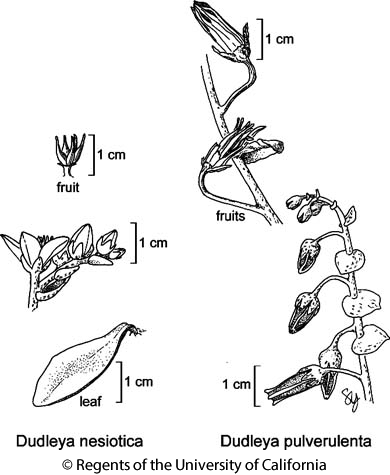
\includegraphics[width=0.6\columnwidth]{figures/fig2-dudleya.png}
\end{center}
\caption{Illustration of \Dudleyanesiotica\ plant \cite{jeps2019dudleya}.}
\label{fig:1.1.2}
\end{figure}






\subsection{Additional Background Research}
We hope to develop innovative methods in the fields of surveying, identification, and object retrieval in places that are difficult to reach. This technology can be refined and tailored for industrial or military in survey and retrieval. 

We looked at the history of air and water temperatures for the environment surrounding the Channel Islands over the past five years during the month of March, our intended operational period. The average air temperature in March has a high of \SI{65}{\fahrenheit} and a low of \SI{49}{\fahrenheit} \cite{accuweather2019channel}. The average water temperature has a high of \SI{58.8}{\fahrenheit} and a low of \SI{53.6}{\fahrenheit} \cite{accuweather2019channel}. In the case where a human person is thrown off the Rigid Hull Inflatable Boat (RHIB) and into the water we have \SIrange{1}{2}{\hour} to rescue them before they develop hypothermia in water conditions from \SIrange{50}{60}{\fahrenheit}. Fog is a common weather feature, especially at San Miguel and Santa Rosa Islands \cite{nps2019weather}. Fog is most common in spring and summer, and west of the Santa Cruz Channel \cite{nps2019weather}. The marine layer fog flows down the coast with the prevailing NW wind, and bends around Point Conception, usually blanketing San Miguel and Santa Rosa, and often the western portion of Santa Cruz Island \cite{nps2019weather}. Fog frequently is thicker and lingers longer into the day offshore than along the mainland coast \cite{nps2019weather}. Preliminary data from Santa Cruz Island suggests that geographic variation in the presence and duration of the fog layer has a profound influence on the temperature and humidity regimes \cite{nps2019weather}. Furthermore, the island chain itself has eight major islands with the largest having an area of \SI{96.51}{\mile\squared} \cite{nps2019weather}. 
\begin{figure}
\begin{center}
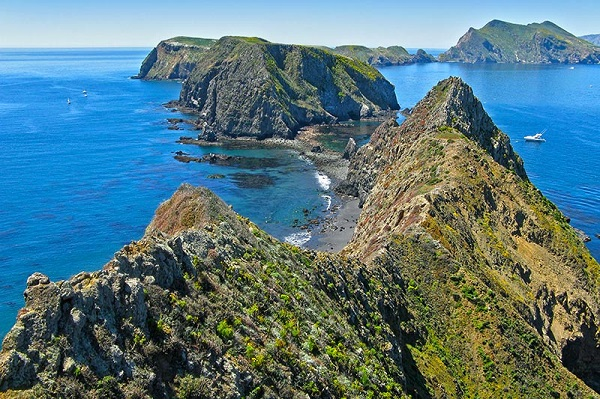
\includegraphics[width=0.8\columnwidth]{figures/fig3-channel.png}
\end{center}
\caption{Aerial Image of the Channel Islands. The larger islands form a National Park which hold many endemic and endangered species of plants \cite{nps2019webpage}.}
\label{fig:1.2.1}
\end{figure}

\begin{figure}
\begin{center}
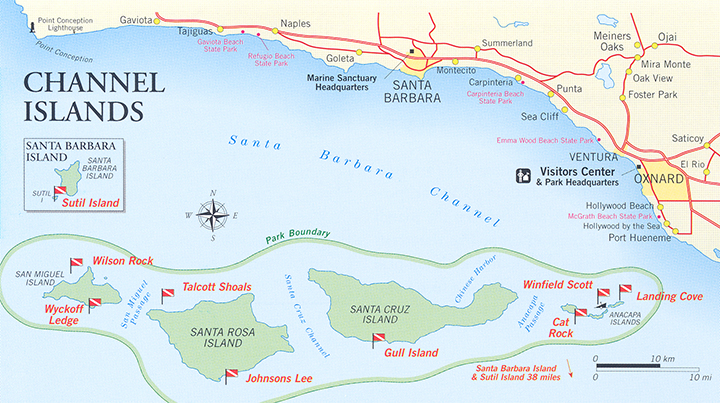
\includegraphics[width=0.8\columnwidth]{figures/fig4-map.png}
\end{center}
\caption{Map of the Channel Islands National Park located 30 miles South of the Santa Barbara Coast \cite{nps2019submerged}.}
\label{fig:1.2.2}
\end{figure}






\section{Problem Statement}
\subsection{Problem Statement}
Our goal is to support the research of Dr. Matthew Guilliams, plant systematist and curator at the Santa Barbara Botanical Garden's Clifton Smith Herbarium, through the survey, extraction, and recovery of the \Dudleyanesiotica\ and \Malvaassurgentiflora, plants endemic to the Channel Islands. Operations will take place near the coastal cliffs of the Channel Islands located off the coast of Santa Barbara. These remote islands are accessible only by boat, and by law, humans are forbidden to step foot on certain islands for environmental protection measures. The two plants of interest are in the vicinity of possibly endangered species, so the team must not harm or disturb the plants surrounding the plant of interest. 

\subsection{Functions}
\begin{figure}
\begin{center}
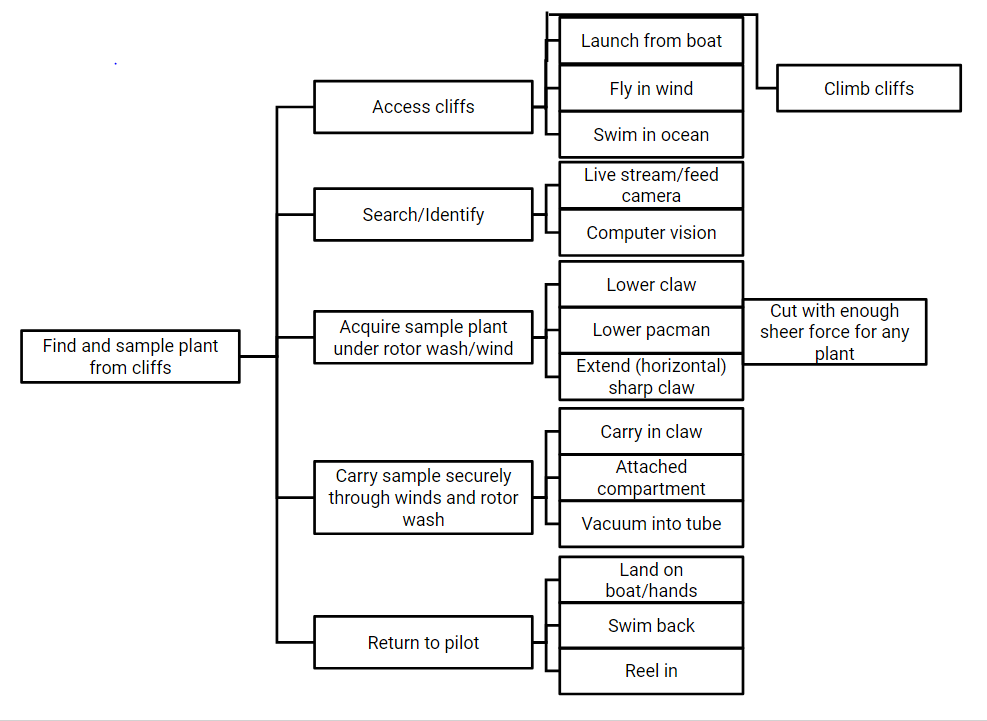
\includegraphics[width=\columnwidth]{figures/fig5-function-tree.png}
\end{center}
\caption{Function Means Tree of the System}
\label{fig:2.2.1}
\end{figure}

\subsection{Constraints}
The average air temperature of the Channel Islands in March is a high of \SI{65}{\fahrenheit} and a low of \SI{49}{\fahrenheit} \cite{accuweather2019channel}. Colder air temperatures will affect the gear needed for operations such as the need for layered clothing, gloves, and thermal insulators for UAS batteries. The average water temperature in March can range from a high of \SI{58.8}{\fahrenheit} and a low of \SI{53.6}{\fahrenheit} \cite{nps2019weather}. If water temperatures are low and the air temperatures are high, there is a high chance for fog which may potentially decrease the field of vision. Severe fog will affect vision and could lead to modification or cancellation of UAS operations. If water temperatures are high, there may be an increase in humidity that will affect the UAS system. Safety during UAS operations are a top priority, thus we must follow safety protocol to ensure no one in the team is at risk for injury or death. As sea state is another factor that will affect RHIB operations, the UAS operations must be done in Channel Island locations with low sea state conditions to ensure optimal operational success. The operational environment is different from a typical flat ground environment in which the Channel Islands’ geography is full of rugged terrain and cliffs. The plants of interest are usually found along the slanted cliffs of the islands, thus we must take into consideration of how the UAS will be designed to ensure the best chances of success in extracting and securing plant samples. 

The landing platform for the UAS operations will be conducted from a RHIB. There will be a limited amount of space for takeoff and landing. There will need to be room for the whole group (five personnel) and a botanist/scientist.  The system must be capable of VTOL (Vertical Takeoff and Landing). In terms of the time period for operation, UAS operations must be conducted during daylight. If there is a day where we cannot fly, there is no way to make up the time by flying at night. The UAS operation cannot damage the environment or other species as the species may be endangered. If the operations were to fail, we must make sure that the UAS will not crash into the island and destroy nature.  Also, one must know when extracting a sample is the appropriate action. For safety of team during RHIB operations, UAS take off, and UAS landing, since the UAS will be taking off and landing on the RHIB, we must make sure that we create and practice a specific and reliable procedure. A constraint concerning securing sample is when the UAS is returning to RHIB, it can be difficult with rotor wash and wind. 

\subsection{Objectives, Pairwise Comparison Chart, and Weightings} 
\begin{table}
\caption{Objective Table split into two portions: mobility and extraction. Objectives for Mobility portion: Part of the system that makes the plant accessible}
\label{tab:2.4.1}
\begin{center}
%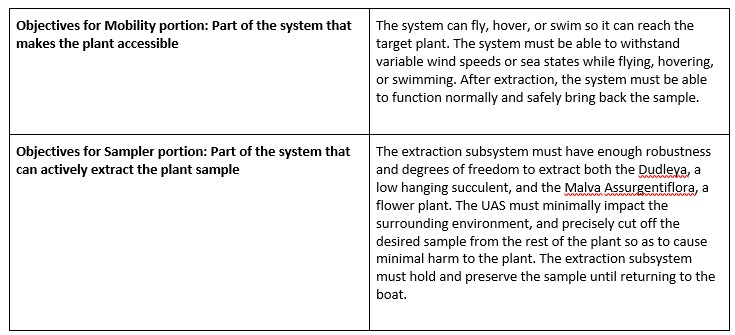
\includegraphics[width=\columnwidth]{figures/table-241.jpg}
\begin{tabular}{p{0.5\columnwidth}p{0.5\columnwidth}}
\toprule
Objectives for Mobility portion: Part of the system that makes the plant accessible &% 
The system can fly, hover, or swim so it can reach the target plant. The system must be able to withstand variable wind speeds or sea states while flying, hovering, or swimming. After extraction, the system must be able to function normally and safely bring back the sample. \\
Objectives for Sampler portion: Part of the system that can actively extract the plant sample &%
The extraction subsystem must have enough robustness and degrees of freedom to extract both the \Dudleya, a low hanging succulent, and the \Malvaassurgentiflora, a flower plant. The UAS must minimally impact the surrounding environment, and precisely cut off the desired sample from the rest of the plant so as to cause minimal harm to the plant. The extraction subsystem must hold and preserve the sample until returning to the boat. \\
\bottomrule
\end{tabular}
\end{center}
\end{table}

The system can fly, hover, or swim so it can reach the target plant. The system must be able to withstand variable wind speeds or sea states while flying, hovering, or swimming. After extraction, the system must be able to function normally and safely bring back the sample.

Objectives for Sampler portion: Part of the system that can actively extract the plant sample
The extraction subsystem must have enough robustness and degrees of freedom to extract both the \Dudleya, a low hanging succulent, and the \Malvaassurgentiflora, a flower plant. The UAS must minimally impact the surrounding environment, and precisely cut off the desired sample from the rest of the plant so as to cause minimal harm to the plant. The extraction subsystem must hold and preserve the sample until returning to the boat.
\begin{table}
\caption{Pairwise Comparison Chart: each metric was compared to the other metrics to determine weights of each metric based on importance to the system.}
\label{tab:2.4.2}
\begin{center}
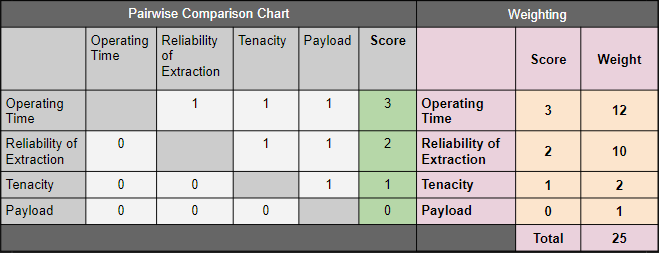
\includegraphics[width=\columnwidth]{figures/table-242.png}
\end{center}
\end{table}



\subsection{Metrics}
Our team developed four metrics to accurately evaluate our design. The metrics are Operating Time, Reliability of extraction, Tenacity, and Total Required Payload. The most important of these metrics is Operating Time since all other metrics depend on the devices ability to successfully operate. Reliability of extraction is the next most important metric since sample extraction is our primary mission.  Tenacity is the third metric due to the environmental factors that must be overcome to accomplish our mission. Lastly our device must have a Payload large enough to support mission necessary equipment.
\begin{table}
\caption{Operating Time Metrics Table}
\label{tab:2.5.1}
\begin{center}
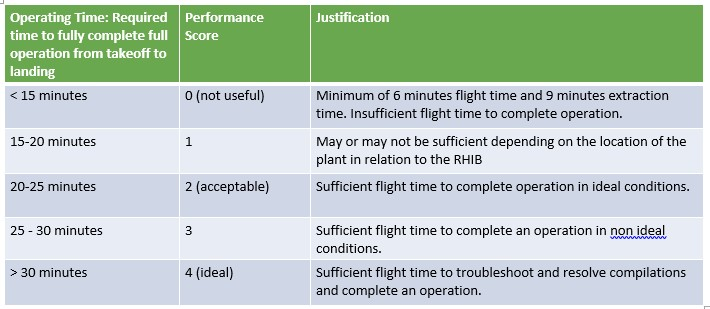
\includegraphics[width=\columnwidth]{figures/table-251.jpg}
\end{center}
\end{table}
\begin{table}
\caption{Reliability of Extraction Metrics Table}
\label{tab:2.5.2}
\begin{center}
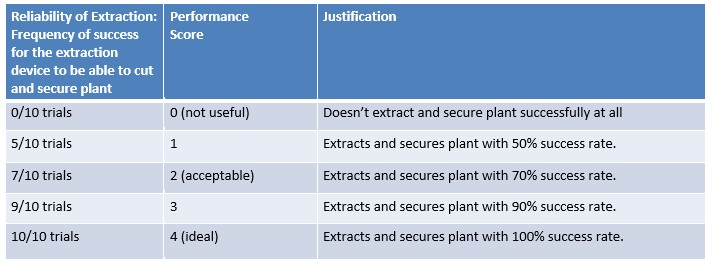
\includegraphics[width=\columnwidth]{figures/table-252.jpg}
\end{center}
\end{table}
\begin{table}
\caption{Total Required Payload Metrics Table}
\label{tab:2.5.3}
\begin{center}
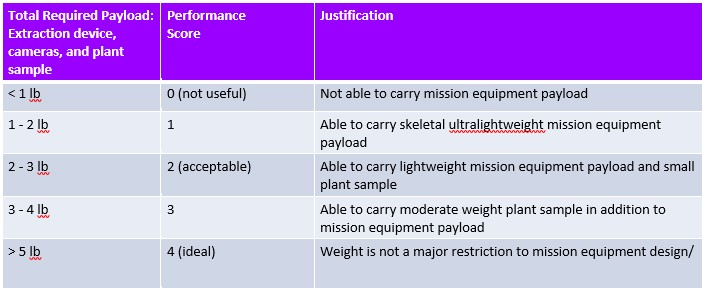
\includegraphics[width=\columnwidth]{figures/table-253.jpg}
\end{center}
\end{table}
\begin{table}
\caption{Tenacity Metrics Table}
\label{tab:2.5.4}
\begin{center}
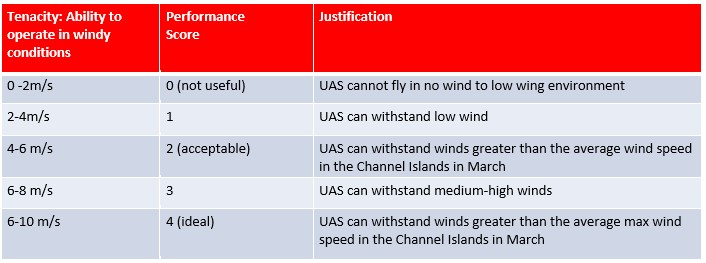
\includegraphics[width=\columnwidth]{figures/table-254.jpg}
\end{center}
\end{table} 






\section{Related Work}
\subsection{National Botanical Garden (NTBG) Plant Survey using UAS}
Ben Nyberg, a UAS operator with NTBG used his UAS to survey and gather footage of plants that are native to Hawaii in hard-to-reach areas.  His job consisted of driving/hiking/helicoptering to the flight location and deploying his UAS.  The average flight time for the UAS ranged from \SIrange{20}{30}{\minute}.  There is usually an assistant with him to help keep the UAS in sight at all times.  All plants are manually identified by the pilot himself during flight operations, and the footage was brought back to other plant experts afterwards.  A big problem that the team ran into was weather.  The islands were very humid and any sort of wind would affect the flight and the control of the UAS \cite{mongabay2019hunting}. 
\begin{figure}
\caption{Picture of Ben Nyberg, a UAS operator with NTBG, using a UAS for surveying \cite{mongabay2019hunting}.}
\label{fig:3.1}
\begin{center}
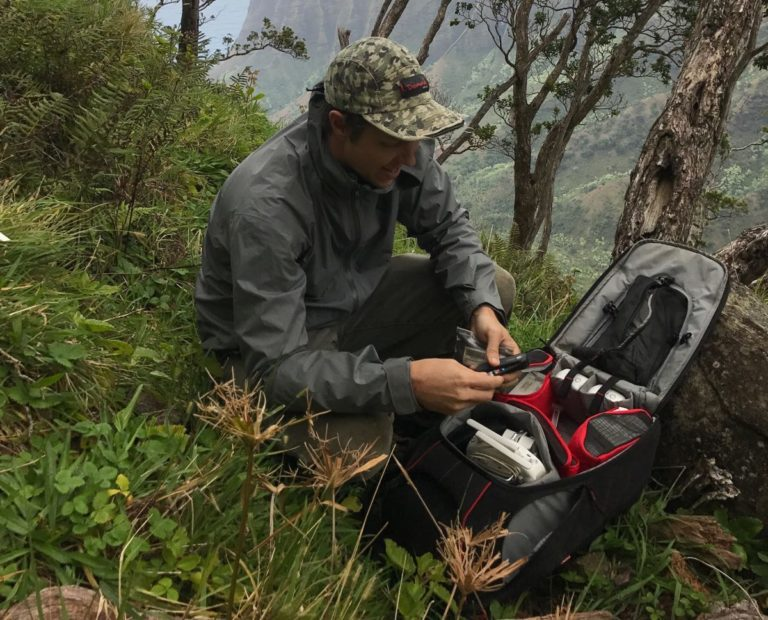
\includegraphics[width=0.8\columnwidth]{figures/fig31-nyberg.png}
\end{center}
\end{figure}

The difference with this design with regards to our mission is that the UAS does not collect samples of the plant and is only used as a means to survey the land. If a species is identified, a professional climber would be airlifted from a helicopter to manually collect the sample. Furthermore, the UAS pilot is able to operate on land where as in our project we will be confined in a RHIB. 

In our design, we would like to create a UAS that can survey the land to identify the desired plants and sample them so that samples do not have to be retrieved manually.  We are also trying to attach additional batteries to our UAS so that the flight time will be increased. A key takeaway from Ben Nyberg’s research is how his team was able to overcome environmental disturbances and compare similarities to that of the Channel Islands. 

\subsection{University of California, Santa Barbara Sampler UAS}
A capstone project of the Mechanical Engineering department of the University of California, Santa Barbara, created a UAS that can fly and take samples of plants.  Their main problem to solve was taking samples of plants in hard-to-reach places using an arm that dangled below the UAS.  The main plants that were sampled were branches of tall trees.  The design that was used can be seen below.
\begin{figure}
\caption{UCSB design for sampler UAS \cite{dantonio2018sampler}.}
\label{fig:3.2}
\begin{center}
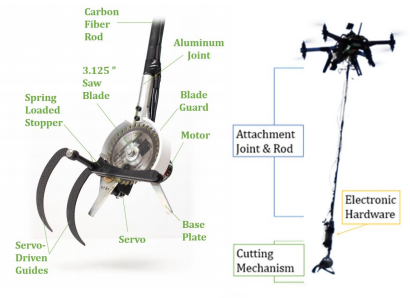
\includegraphics[width=0.8\columnwidth]{figures/fig32-ucsb.png}
\end{center}
\end{figure}

Issues with this design with regards to our mission: Average flight time of \SI{7}{\minute}; Made to cut larger branches; The control of the UAS greatly affected the quality of the sample; Octocopter was used instead of a quadcopter.

Although a working design, the UCSB capstone design was unable to fly for our minimum flight time of \SI{15}{\minute}.  The design also is not ideal for sampling plants that are growing on near-vertical cliffs because the UAS would not be able to position itself directly overhead of the plant. 

\subsection{Airborne refueling probe basket}
The military uses a system called a probe-and-drogue which employs a hose from a tanker aircraft with a drogue (a funnel-like basket) attached to the end of the hose in order to catch the probe on the receiving aircraft.  The basket is made to be drag-resistant and sturdy enough to guide the probe into the nozzle \cite{ren2019reliable}.    
\begin{figure}
\caption{Picture of Airborne refueling probe basket \cite{ren2019reliable}}
\label{fig:3.3}
\begin{center}
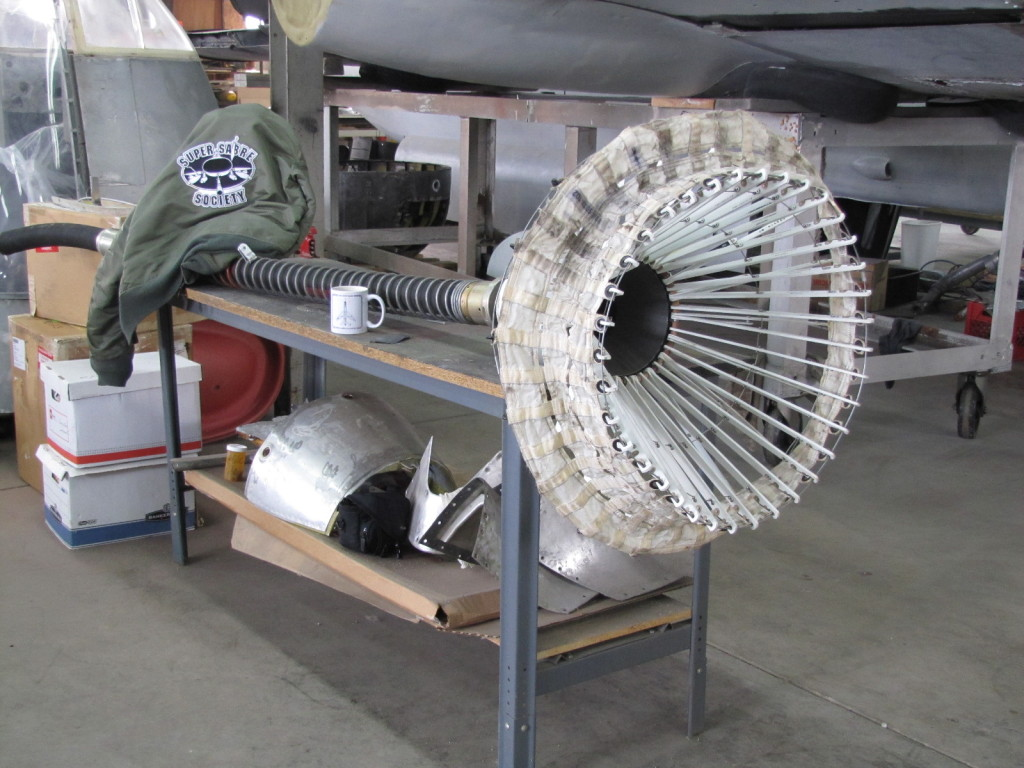
\includegraphics[width=0.8\columnwidth]{figures/fig33-refueling.png}
\end{center}
\end{figure}

This type of design is helpful for the snipper/gripper design because this will help guide the plant into the hole where it can be cut and stored.  However, funneling a plant is different than guiding a fuelling probe.  The refuelling drogue is made to fly backwards while our fixture is facing into the direction of flight.  In our design we incorporated a cone-shaped mesh to help funnel a branch into the cutting zone.





\section{Conceptual Designs}
When reviewing the customer requirements and overall objectives our team was able to derive definitive functions for our conceptual  designs. Overall we want to develop an unmanned UAS system that is able to survey an island, search and identify a species of plant and recover with minimal interference to the plant themselves. Circled red on our morth chart are viable solutions to respective functions. The conceptual design below integrate technologies annotated in the morph chart.
\begin{table}
\caption{Overall Morth Chart with all viable capabilities}
\label{tab:4.1}
\begin{center}
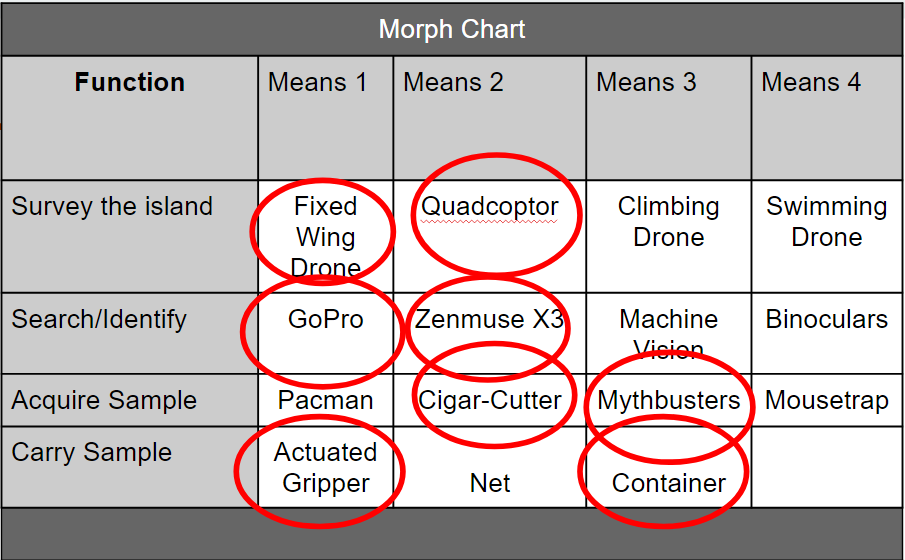
\includegraphics[width=\columnwidth]{figures/table-41.png}
\end{center}
\end{table}


\subsection{Concept 1: Quadcopter Survey and Extraction}
The first concept that was evaluated was the Quadcopter Survey and Extraction. The UAS will only have a camera system when surveying to maximised flight time. Currently we are working with the DJI Matrice 100 and the Zenmuse X3 camera and gimbal \cite{dji2019zenmuse}.  The maximum hovering time of with two batteries, gimbal and camera set up is \SI{30}{\minute} giving us a 3/4 on our operating time matrics \cite{dji2019dji}. \SI{30}{\minute} gives sufficient flight time to complete an operation in non ideal conditions as well as flexibility when surveying island cliffs. While \SI{30}{\minute} is not much time, it's on average higher than other quadcopters of its size and capability. Furthermore the Matrice 100 is able to fly in a maximum of \SI{22}{\mph} wind conditions \cite{dji2016m100}.

With the maximum winds of the Channel Islands in March being \SI{18}{\mph} this system scored a 4/4 on our tenacity metric.  After launching from the RHIB, the UAS will follow waypoints around the perimeter of the island and utilize a camera system to record the cliffside. Once sufficient video is taken or a low power mode is activated the UAS will return back to the RHIB where our team will extract the footage for review.  After reviewing the footage if there is a plant species that needs to be collected we will attach, in addition to the Zenmuse X3 gimbal, our extraction system. 

The Matrice 100 has an estimated maximum payload of \SI{1.15}{\kilo\gram} for one battery excluding the weight of that battery. The maximum weight for two batteries needs to be tested given the extra battery weighs \SI{672}{\gram}. Currently we give the Matrice a  2/4 acceptable rating in our total required payload metric which includes extraction device, camera and plant sample. The Zenmuse X3 and gimbal’s weight is \SI{247}{\gram} giving our team the remander \SI{868}{\gram} to work with. We will release the Matrice, use the extraction system to collect a sample of the plant and return back to the RHIB successfully. The conceptual design of the extractors will be discussed later in this section.  
\begin{figure}
\begin{center}
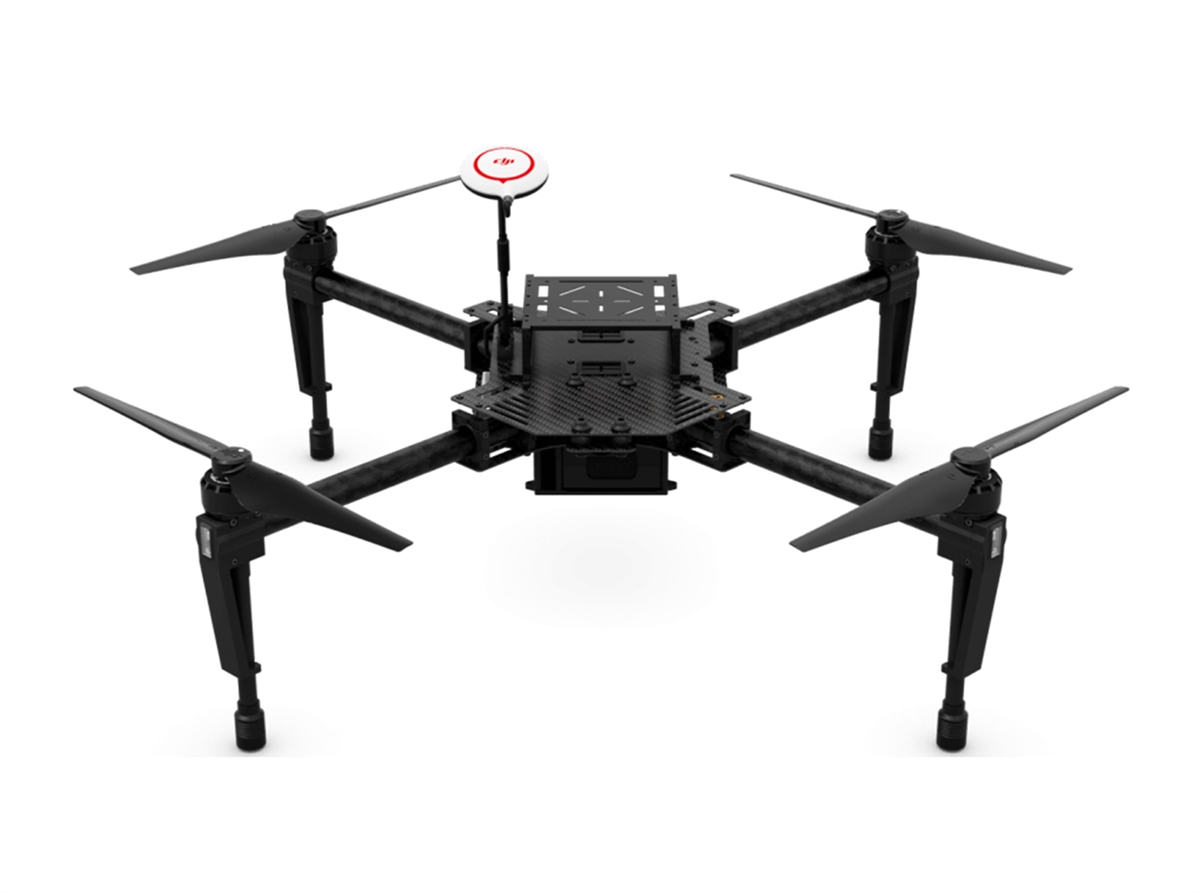
\includegraphics[height=1.3in]{figures/fig411a.png}
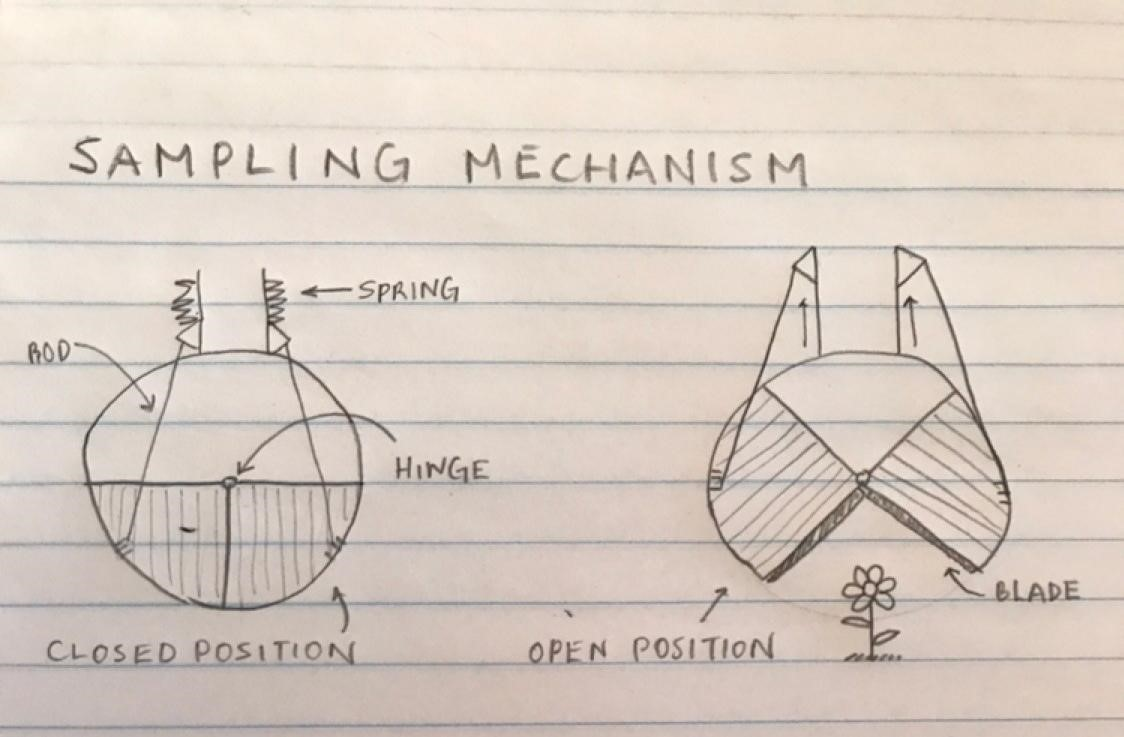
\includegraphics[height=1.3in]{figures/fig411b.jpg}
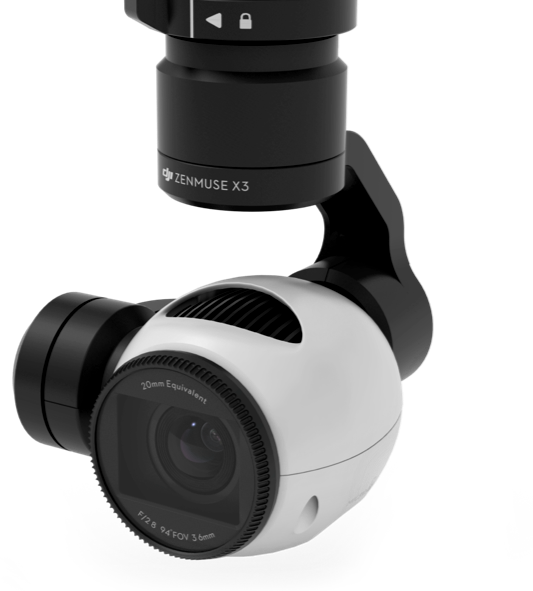
\includegraphics[height=1in]{figures/fig411c.png}
\end{center}
\caption{DJI Matrice 100, Prototype Drawing of Extraction Mechanism, and Zenmuse X3 Gimbal respectively \cite{dronesmadeeasy2019matrice, dji2019zenmuse}.}
\label{fig:4.1.1}
\end{figure}



\subsection{Concept 2:  Fixed-Wing Quadrotor Combo}
The second concept that was evaluated was the Fixed-Wing Quadrotor Combo. The Fixed Wing UAS would be used for the initial steps of surveying the island to search and identify the respective plant species. On average the operating time of fixed wing aerial systems is \SI{45}{\minute} giving the Operating Time metric a 4/4. \SI{45}{\minute} gives sufficient time to troubleshoot complications if arise and complete the operation. The payload of the Fixed Wing UAS is not as important because there are usually built in cameras. Whereas the payload and overall specifications of the Quadcopter will be the same as in concept one. The Matrice 100  would be sent out to desired plant location for extraction due to its higher stability. The pros of incorporating the fixed wing UAS would be an estimated 50\% increase in operating time and potentially high video quality. The downside would be purchasing/acquiring a whole new system, learning how to use it and takeoff/landing procedures. We looked at the WingtraOne, a fixed wing UAS developed by Wingtra \cite{wingtra2019wingtraone}. The Wingtra has no listed price but camera offers a minimal ground sampling distance of \SI{0.7}{\centi\meter} and vertical take off and landing \cite{wingtra2019wingtraone}. 

\begin{figure}
\begin{center}
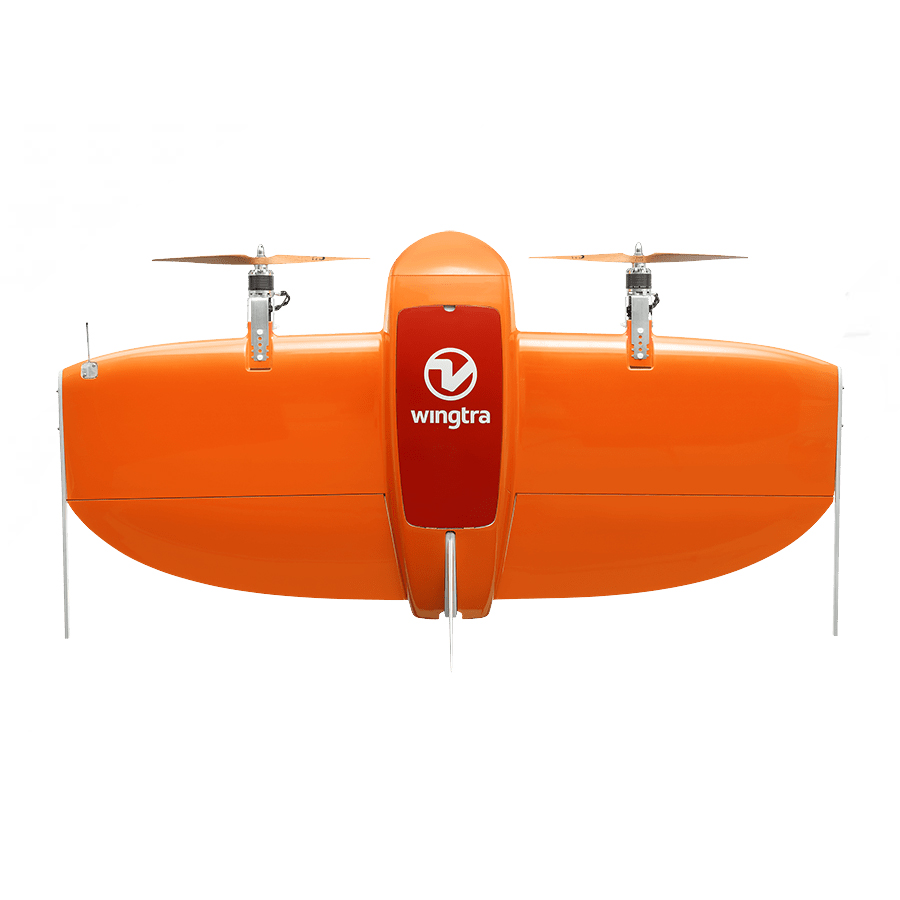
\includegraphics[height=1in]{figures/fig421a.png}
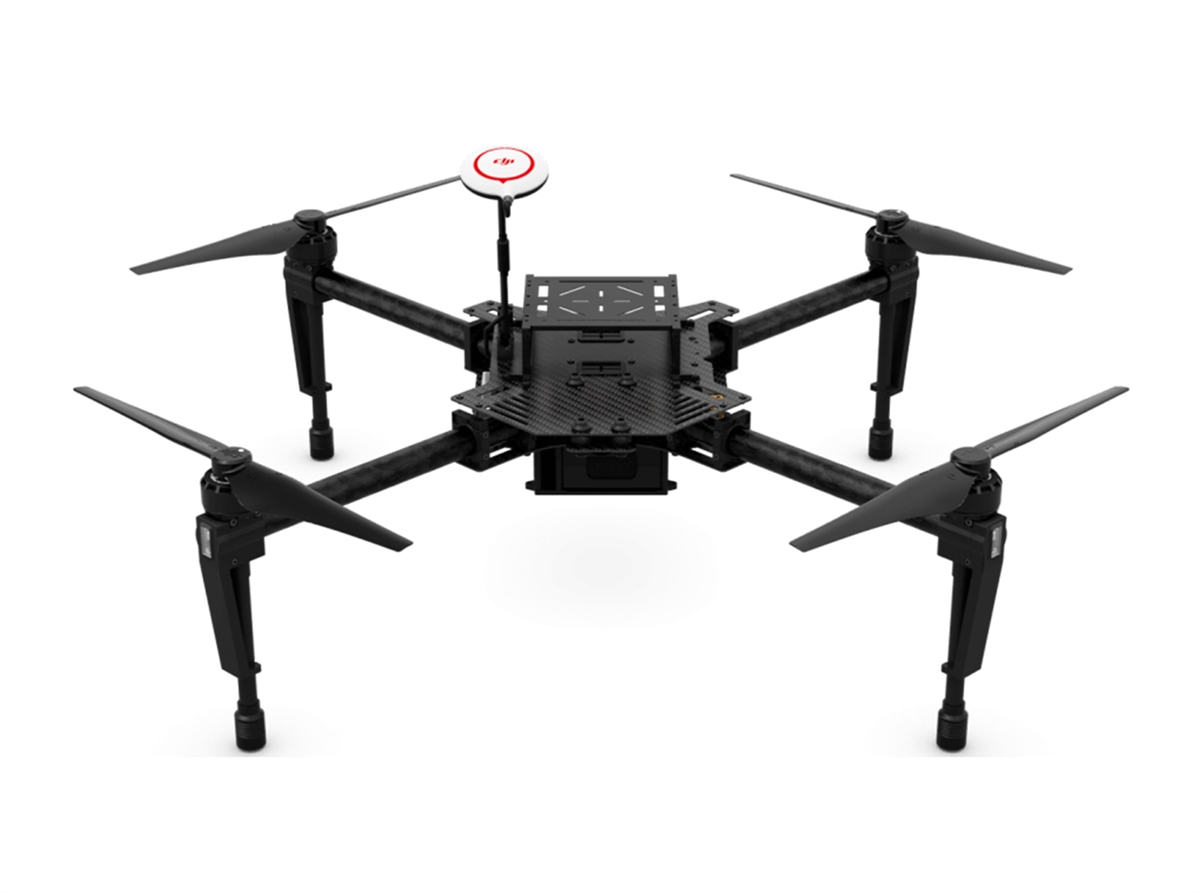
\includegraphics[height=1in]{figures/fig421b2.png}
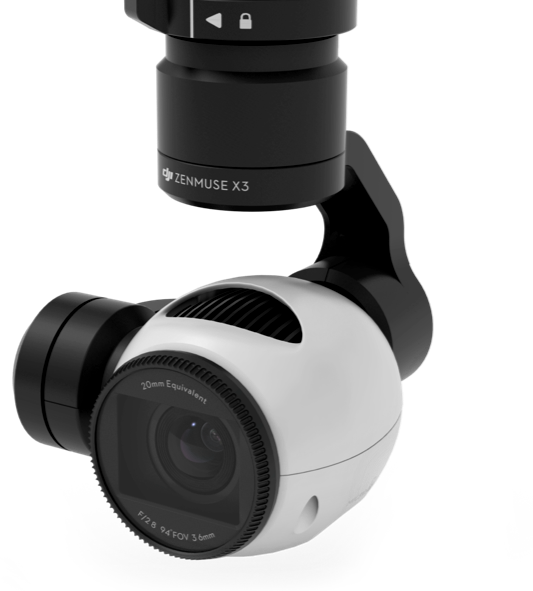
\includegraphics[height=0.2in]{figures/fig421b1.png}
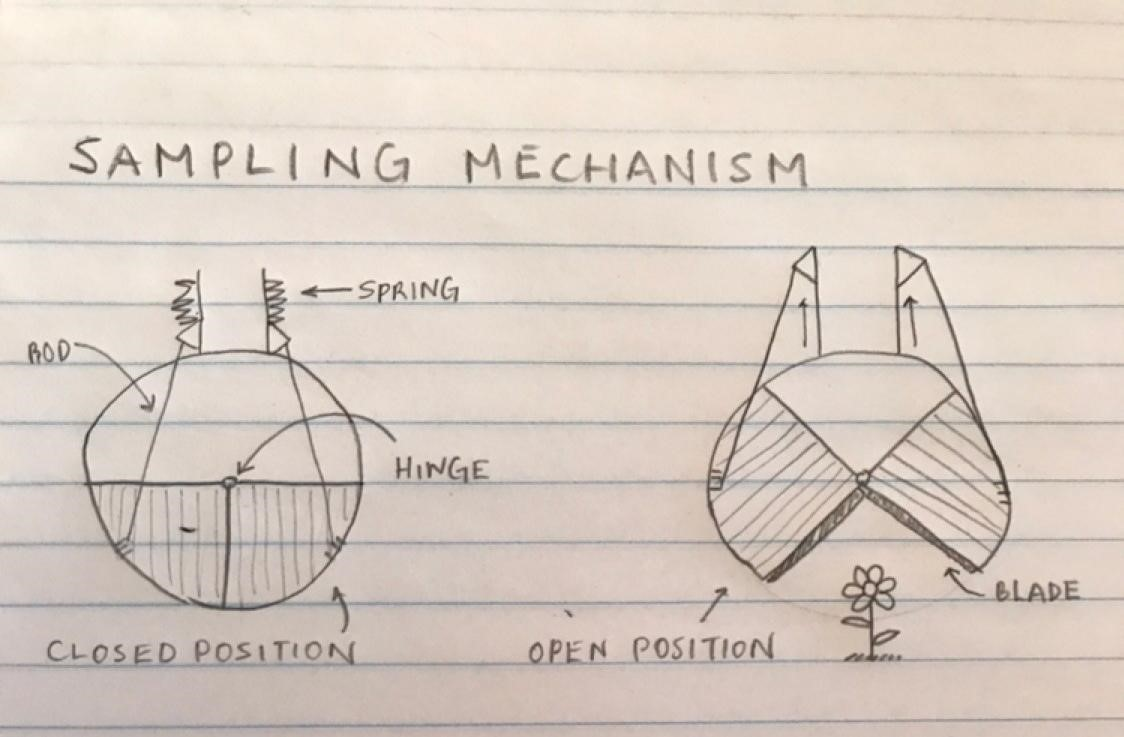
\includegraphics[height=0.8in]{figures/fig421c.jpg}
\end{center}
\caption{Fixed-wing UAS, DJI Matrice 100 with Zenmuse X3 Attached, and Prototype Drawing of Extraction Mechanism respectively  \cite{dronesmadeeasy2019matrice, wingtra2019wingtraone, dji2019zenmuse}}
\label{fig:4.2.1}
\end{figure}





\subsection{Concept 3:  Climbing Robot}
Robot with Four Servo legs that is able to climb onto steep rocky cliffs and be able to extract plant sample through extraction device beneath the robot. The benefits of this design are its operating time, payload and tenacity. The robot itself needs to be transported onto the island via quadcopter. Because the robot is constricted to the ground and limited in movement its use for surveying the island to search and identify plants would be futile. Whereas recovering the plant would not be, given that a ground system does not need to adhere to the same physics as our air counterparts we will be able to attach a hefty payload and in turn maximise our operating time.  Cliff Climbing Robots are built with hook like claws to attach to rocky surfaces and potentially with anti-vibration and anti-wind loading. The robot will be able to withstand the highest winds speed of the channels island scoring highest in our tenacity metric. While  these ideas are great in theory, developing a whole robotic cliff climbing robot is beyond our capabilities  and level of experience. Furthermore, the system that delivers the UAS must provide a payload that can withstand the weight of the robot. 
\begin{figure}
\begin{center}
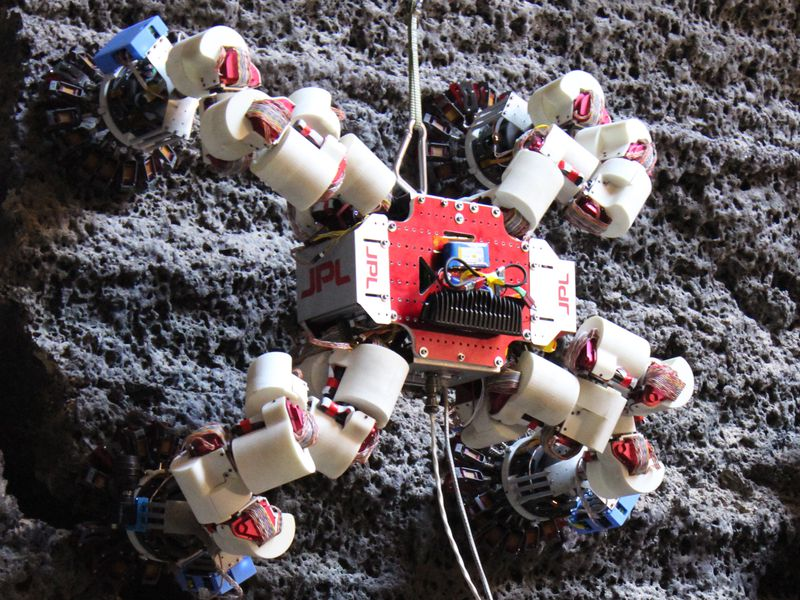
\includegraphics[width=0.5\columnwidth]{figures/fig431.png}
\end{center}
\caption{NASA JPL Lemur 3 Climbing Robot \cite{donahue2017new}}
\label{fig:4.3.1}
\end{figure}



\subsection{Concept 4: Cigar-Cutter Extraction Mechanism}
This extraction system utilizes spring power over a cigar cutter to cut the plant. It is strategically placed behind a cone and before a clear tube so that once the spring mechanism is activated it will not only cut the plant but also trap it in the tube, securing the plant inside the tube for recovery. There will be a camera that points to the clear tube so that the UAS co-pilot will know when to activate spring loaded trap while the main UAS pilot can focus on positioning the UAS during the extraction process. This system is predicted to work 5/10 trials. This is not because the cutter will not cut through  the plant, but the limitation of if the plant does not go into the cone all the way and the spring is activated. Another limitation is that the cigar-cutter is one try method because the cigar cutter cannot be reset unless the UAS returns to the boat and physically reset by hand. 
\begin{figure}
\begin{center}
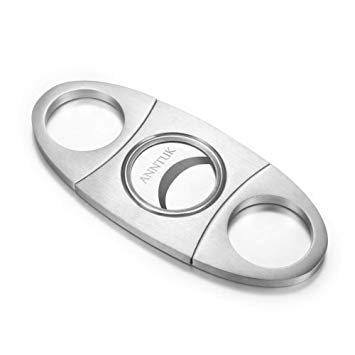
\includegraphics[width=0.5\columnwidth]{figures/fig441.png}
\end{center}
\caption{Sample picture of cigar cutter used for design \cite{famoussmoke2019cigar}}
\label{fig:4.4.1}
\end{figure}





\subsection{Concept 5: Mythbuster Motorized Shear}
Developed by Mythbusters host Jamie Hyneman, the motorized shear uses a high torque motor and a worm drive gear orientation to translate a motor’s single axis spin into planar rotational motion. The planar circular motion controls the end effector shears to repeatedly open and close at a comfortable speed. In the video, Jamie Hyneman demonstrates how powerful the shears are by easily cutting through thick branches, and then proceeds to attach the subsystem to his UAS. He flies the UAS to a bush and begins cutting branches off \cite{mbed2019}. This is exactly the kind of design that we envision.
\begin{figure}
\begin{center}
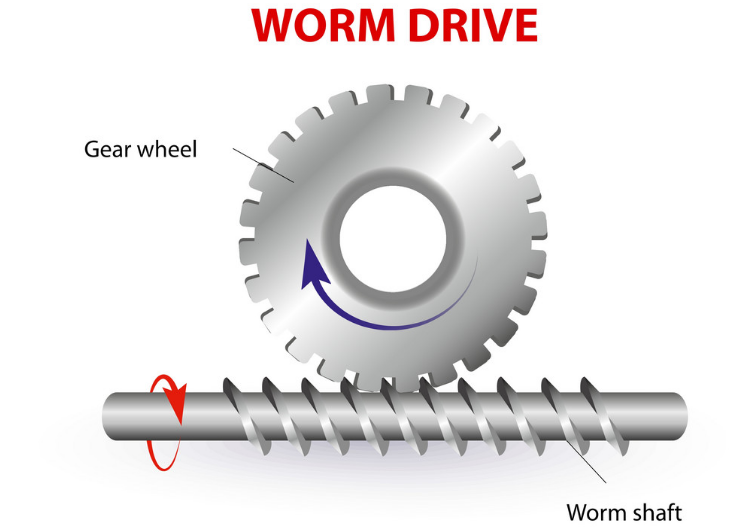
\includegraphics[width=0.5\columnwidth]{figures/fig451.png}
\end{center}
\caption{Worm drive diagram that shows how axis rotation can be translated into rotational planar motion \cite{wikipedia2019wormdrive}.}
\label{fig:4.5.1}
\end{figure}
\begin{figure}
\begin{center}
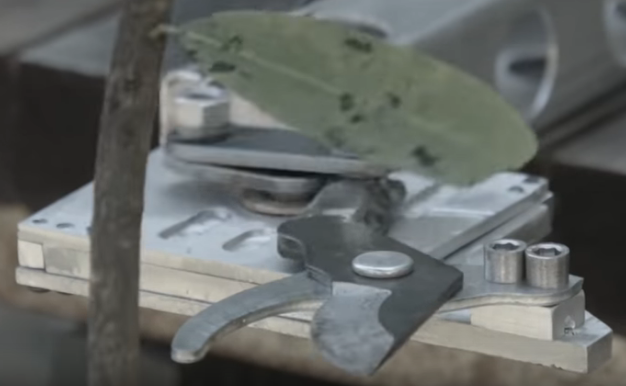
\includegraphics[width=0.4\columnwidth]{figures/fig452.png}
\end{center}
\caption{The end effector of the motorized shear \cite{mbed2019}.}
\label{fig:4.5.2}
\end{figure}







\subsection{Decision Matrix}
\begin{table}
\caption{Decision Matrix Chart}
\label{tab:4.6.1}
\begin{center}
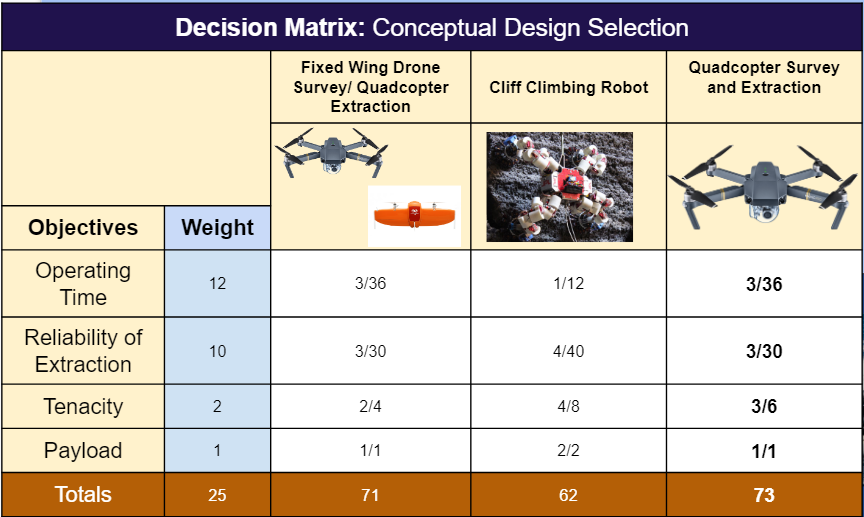
\includegraphics[width=\columnwidth]{figures/table-461.png}
\end{center}
\end{table}

\Fref{tab:4.6.1} shows our analysis of comparing all three he designs. While the single quadcopter design scored the highest, the Fixed Wing UAS Survey with Quadcopter Extraction came in a close second. The only difference in the matrix of these is that the single UAS system is less complex and therefore has less room for failure. The Climbing Robot involves too many additional pieces needed such as a way to send out and retrieve the robot after a successful extraction. We speculate the Climbing Robot to be the most reliable in extraction, but operating a robot from afar on a boat seems much too difficult. Though the single quadcopter design won in terms of points on the decision matrix, our group has still not given up on the idea of a quadcopter and fixed wing project. During the first semester, we focused on the extraction and flying elements of the quadcopter because it is the quadcopter that will ultimately do the extraction. We plan to incorporate testing with a fixed wing UAS for survey purposes.

\begin{figure}
\caption{Functional Block Diagram of the DJI M100 with a Motorized End Effector}
\label{fig:4.6.1}
\begin{center}
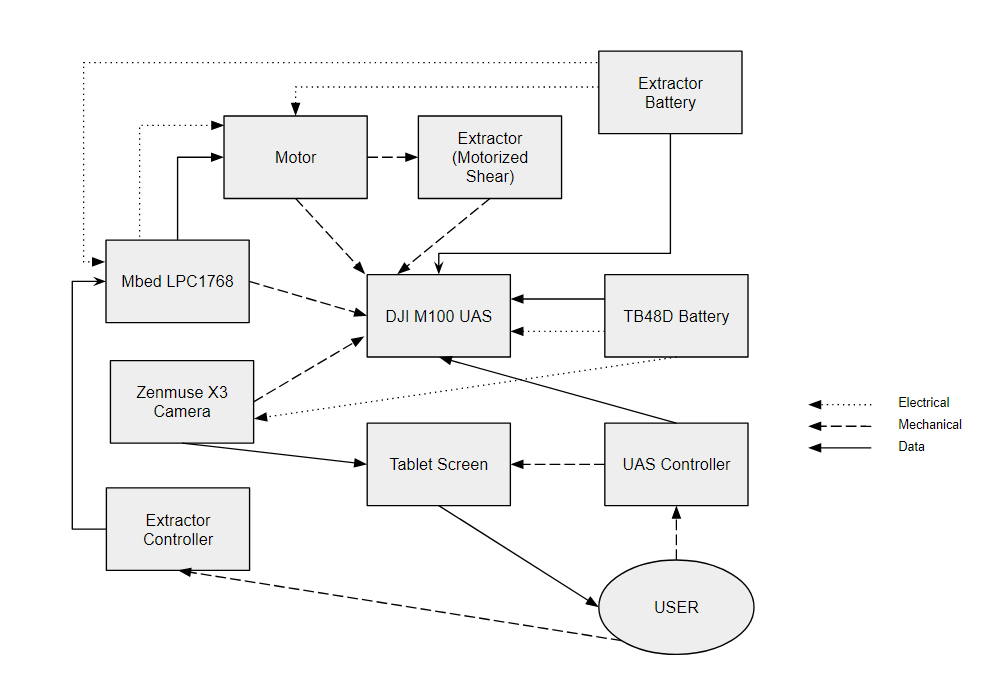
\includegraphics[width=\columnwidth]{figures/fig461.png}
\end{center}
\end{figure}







\section{Ethical Considerations}

Our project inherently contained a lot of space restrictions, and the nature of the mission has many restrictions placed by the Environmental Protection Agency (EPA).  A primary ethical concern for our project is nested in the act of damaging endangered species.  In order to retrieve a sample of an endangered species, it must be damaged.  This goes against the Endangered Species Act (ESA) of 1973 which states that endangered species cannot be carried, delivered, received, or shipped \cite{czech2001endangered}.  The act also states that endangered species cannot be damaged or destroyed in knowing violation of any law.  The Santa Barbara Botanical Garden has a permit to invade these islands and collect the samples.  As a team, we must make sure that, even though we have permission to damage the endangered plant life, we keep the damage to a bare minimum.  As a team, we must make sure that the assurances we make are honest and realistic to ensure that there is no miscommunication of expectations between us and the customer (for example: if our system is likely to damage to  the plant and the surrounding cliff, we must be clear about it).  This complies with the Institute of Electrical and Electronics Engineers (IEEE) Code of Ethics.  During testing, there may be times when we are forced to make a decision between the safety of ourselves or the safety/success of the mission.  For example, when landing the drone on the boat, team members may reach out to grab the drone if it looks like it will not stably land on the platform.  This may potentially cause the team member to hurt his/her hand or fall out of the boat.  As a team, we must comply with the IEEE Code of ethics which states that we need to ``hold paramount the safety of the public'' and ``avoid injuring others.''  In order to mitigate this risk, we must understand our own capabilities and only attempt endeavors at which we are most likely to succeed.  Being aware of one’s capabilities and acting within our abilities is emphasized by both the IEEE Code of ethics, and the Profession Engineer’s Code. 





\section{Engineering Standards and Specifications}

\begin{table}
\caption{Lithium Battery Standards Table \cite{mpoweruk2019international}}
\label{tab:6.1}
\begin{center}
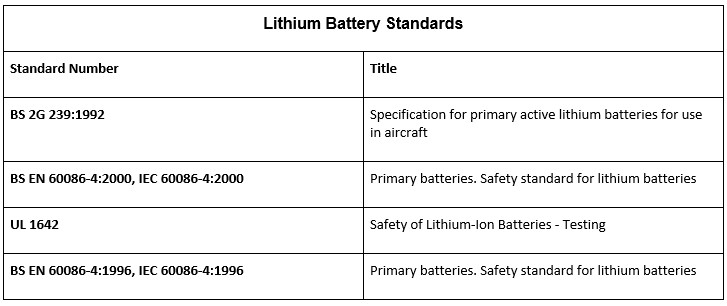
\includegraphics[width=\columnwidth]{figures/table-61.jpg}
\end{center}
\end{table}

Lithium Batteries are a staple in any operation involving UAS because of their high specific energy, extremely advantageous when weight is a constraint. There are numerous standards for lithium polymer battery training, safety, and use in aircraft operations. Our team completed lithium polymer battery training with Professor Evangelista.






\section{Preliminary Detailed Design}
\subsection{Component Selection}
The UAS system we chose to use was the DJI Matrice 100. In respect to our design matrix of ``operating time'' the Matrice 100 offeres us a performance score of acceptable (2/4) providing sufficient time (\SIrange{20}{25}{\minute}) to complete operation in ideal conditions.  We determined the acceptable operating time of \SIrange{20}{25}{\minute} from reviewing the DJI Matrice 100 manual, available battery power of the TD48B smart Batteries and estimated overall payload. The DJI Matrice 100 also satisfies another design matrix ``Total Required Payload'' with a score of acceptable (2/4) being able to carry lightweight mission equipment payload and small plant sample. We determined that the total weight of our payload to include snipper/gripper, attachment system, camera, gimbal and external power should not weigh more than \SIrange{2}{3}{\pound}. Furthermore the DJI Matrice 100 satisfies another design matrice ``tenacity'' the ability to operate in windy conditions with a performance score of acceptable (2/4) able to overcome \SIrange{4}{6}{\meter\per\second} which are greater than average wind speed in the Channel Islands in March.  The camera system we chose to use is the Zenmuse X3. We chose the Zenmuse X3 for our beginning stages of prototyping because it provides us with an extremely user accessible gimbal. The controllable range is tilt \ang{+30} to \ang{-90}, pan \ang{\pm 320} and roll of \ang{\pm 15}. The camera quality itself is descent with 12 megapixels of resolution and $\num{3.5}\times$ zoom. It is able to record at a maximum UDH 4k 25p and has a white balance option for cloudy conditions. Furthermore it has the capacity to store up to 64 gb on a mini SD card. 
        
\subsection{Parts List and Budget}
\begin{table}
\caption{Complete Parts List}
\label{tab:7.2.1}
\begin{center}
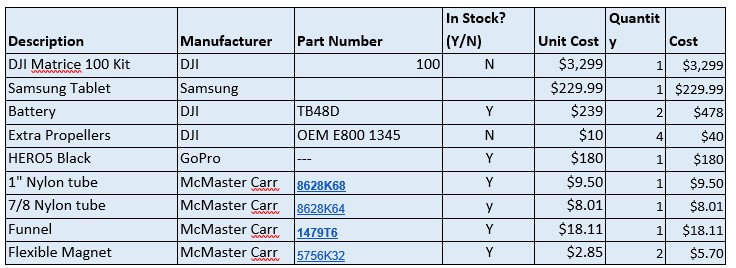
\includegraphics[width=\columnwidth]{figures/table-721.jpg}
\end{center}
\end{table}
\begin{table}
\caption{Complete Budget List. Disclaimer: ``labor'' costs, person-day rates, and ``overhead'' are fictional and are solely for EW401 training purposes. They do not reflect actual costs.}
\label{tab:7.2.2}
\begin{center}
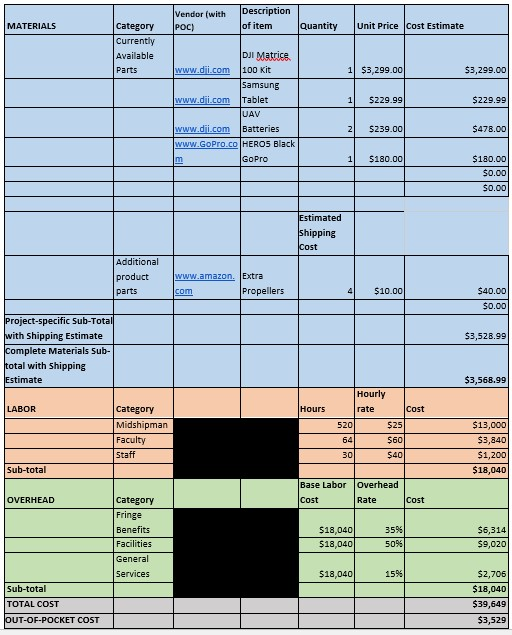
\includegraphics[width=\columnwidth]{figures/table-722.jpg}
\end{center}
\end{table}





\subsection{Mechanical Drawings}

\begin{figure}
\begin{center}
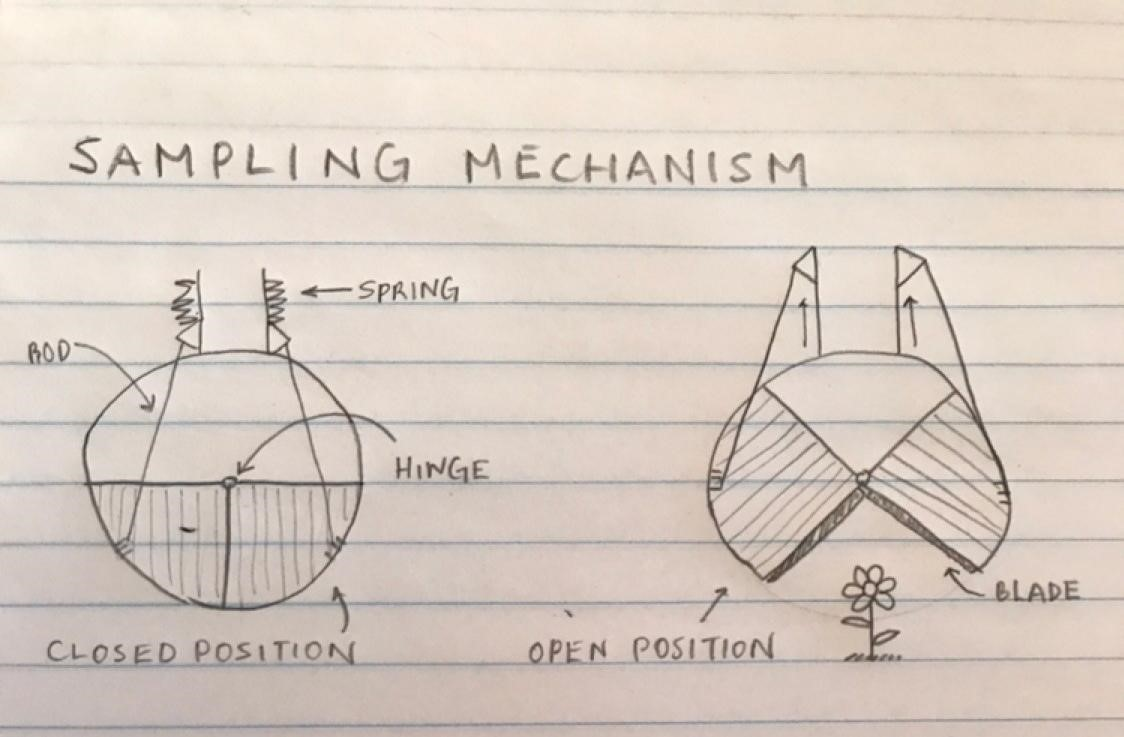
\includegraphics[width=0.8\columnwidth]{figures/fig731.jpg}
\end{center}
\caption{A prototype drawing of the initial Pac-Man design for extraction}
\label{fig:7.3.1}
\end{figure}
Initially, a grabber system that resembled a video game character, Pac-Man, was contemplated.  The apparatus would be attached to the end of a long rod attached to the UAS, and actuated by a solenoid.  The design incorporated blades on the sliding hatches that were pushed closed by strong springs that were attached to the rod portion.  For simplicity, and conservation of weight, the design was a strong, single-cut (one and done). 

After some rumination, the Pac-Man design was altered in order to have less moving parts.  The second design looked more like the mouth of an eel.  Unlike the two moving hatches of the initial design, the new grabber system was designed with a fixed bottom jaw which would act like an anvil to the blade attached to the top jaw.  The top jaw would be snapped closed using tension from strong torsion springs similar to those found in a household mousetrap.
\begin{figure}
\begin{center}
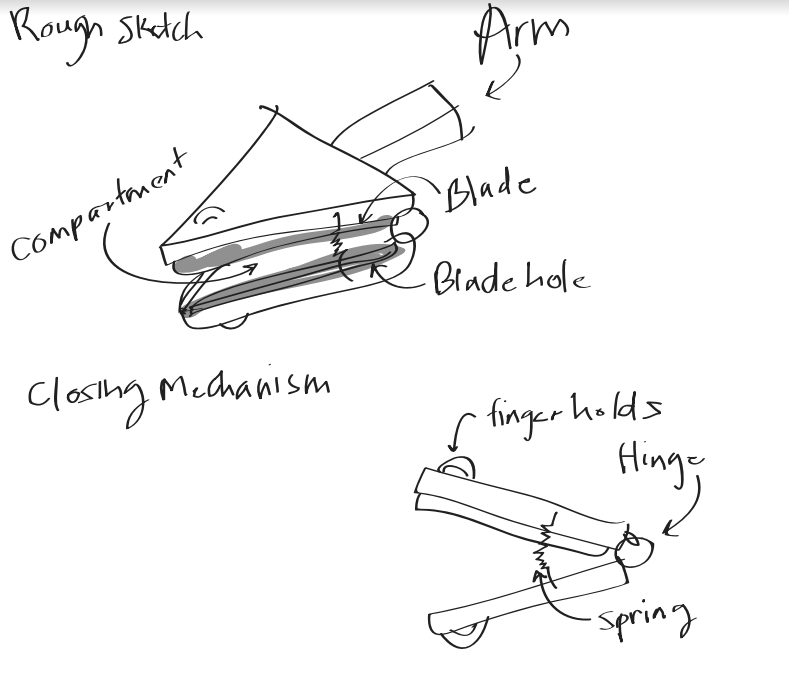
\includegraphics[width=0.6\columnwidth]{figures/fig732.png}
\end{center}
\caption{A rough sketch of the revised Pac-Man design}
\label{fig:7.3.2}
\end{figure}

\begin{figure}
\begin{center}
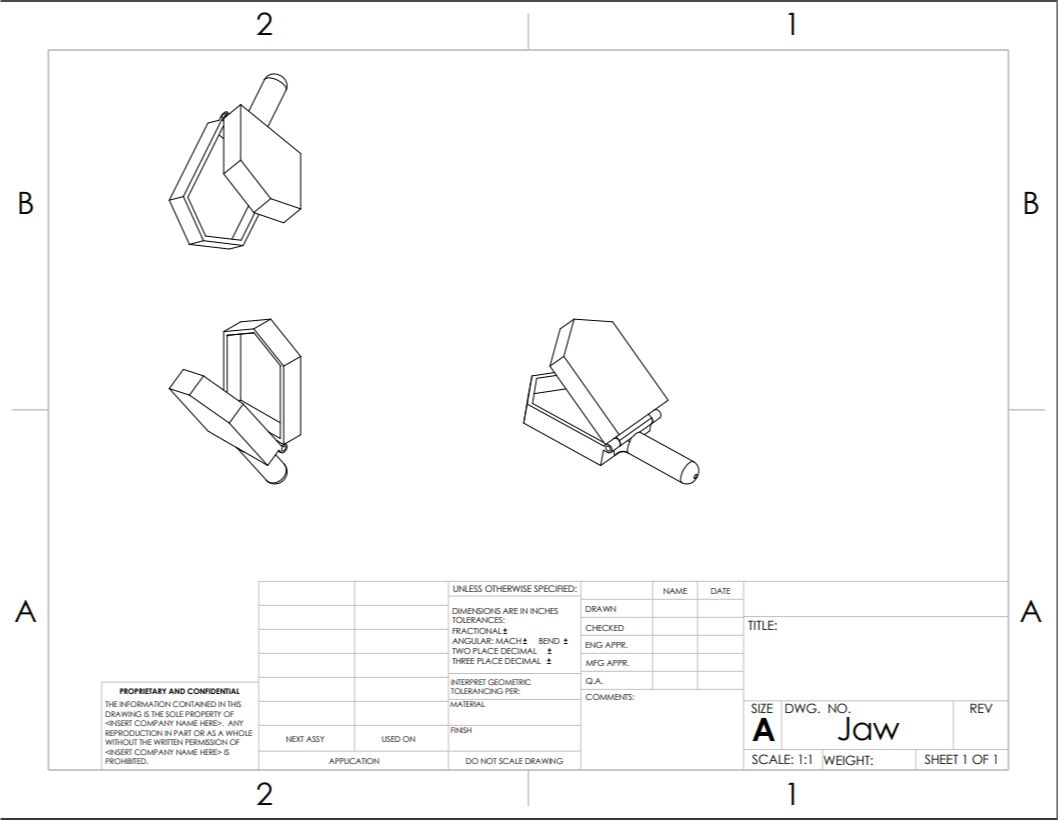
\includegraphics[width=0.8\columnwidth]{figures/fig733.png}
\end{center}
\caption{A digital drawing of the new Pac-Man design}
\label{fig:7.3.3}
\end{figure}

\begin{figure}
\begin{center}
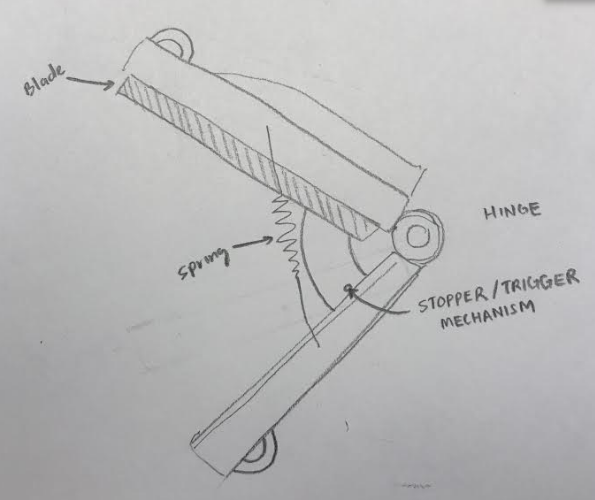
\includegraphics[width=0.8\columnwidth]{figures/fig734.png}
\end{center}
\caption{Prototype sketch of revised pac man design with parts labelled}
\label{fig:7.3.4}
\end{figure}

The location for the cutter system had to be outside of the rotor wash generated by the rotors that were closest to it.  Therefore, it was decided that the bar would extend about \SI{500}{\milli\meter} from the drone center (\fref{fig:7.3.5}). 
\begin{figure}
\begin{center}
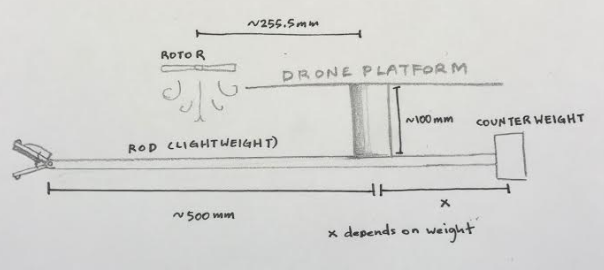
\includegraphics[width=\columnwidth]{figures/fig735.png}
\end{center}
\caption{Prototype drawing of complete pac man design}
\label{fig:7.3.5}
\end{figure}
 
After discussing the Pac-Man design with the workers at the Machine Shop, it was decided that the 
\begin{figure}
\begin{center}
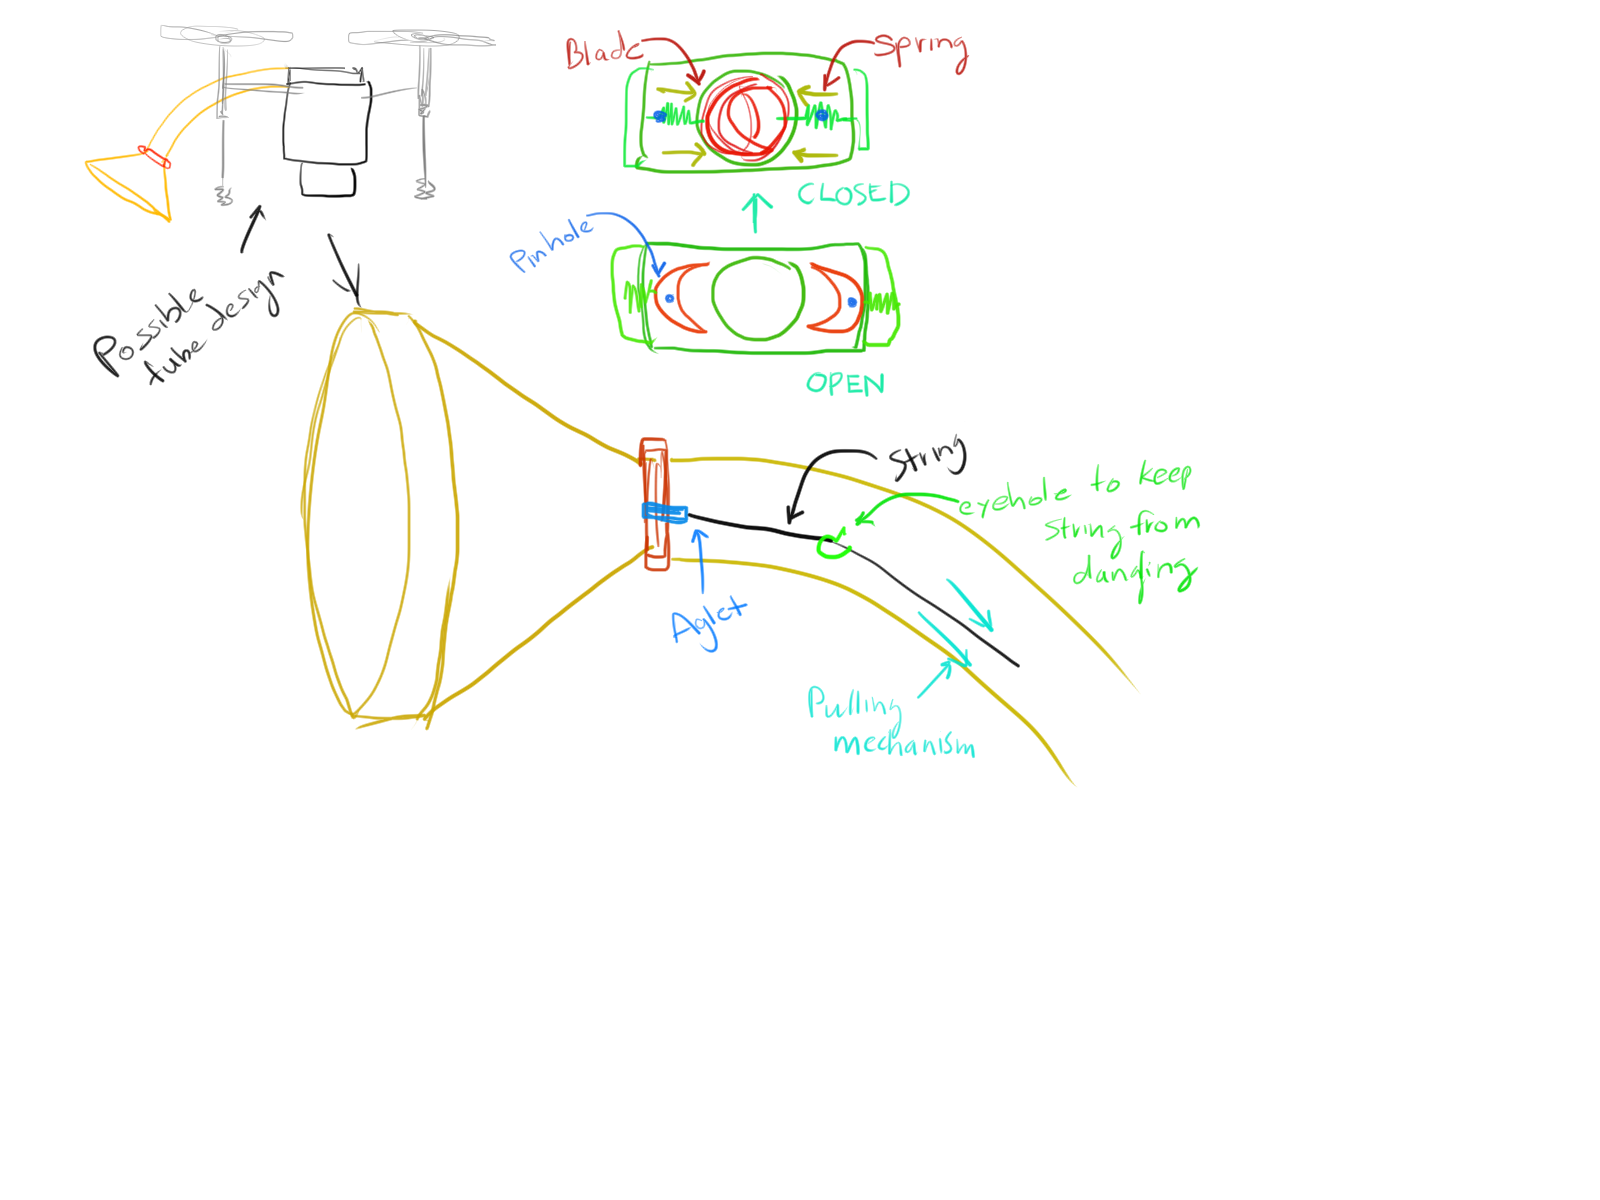
\includegraphics[width=\columnwidth]{figures/fig736.png}
\end{center}
\caption{Initial prototype drawing of cigar cutter extraction mechanism with tube and cone}
\label{fig:7.3.6}
\end{figure}
\begin{figure}
\begin{center}
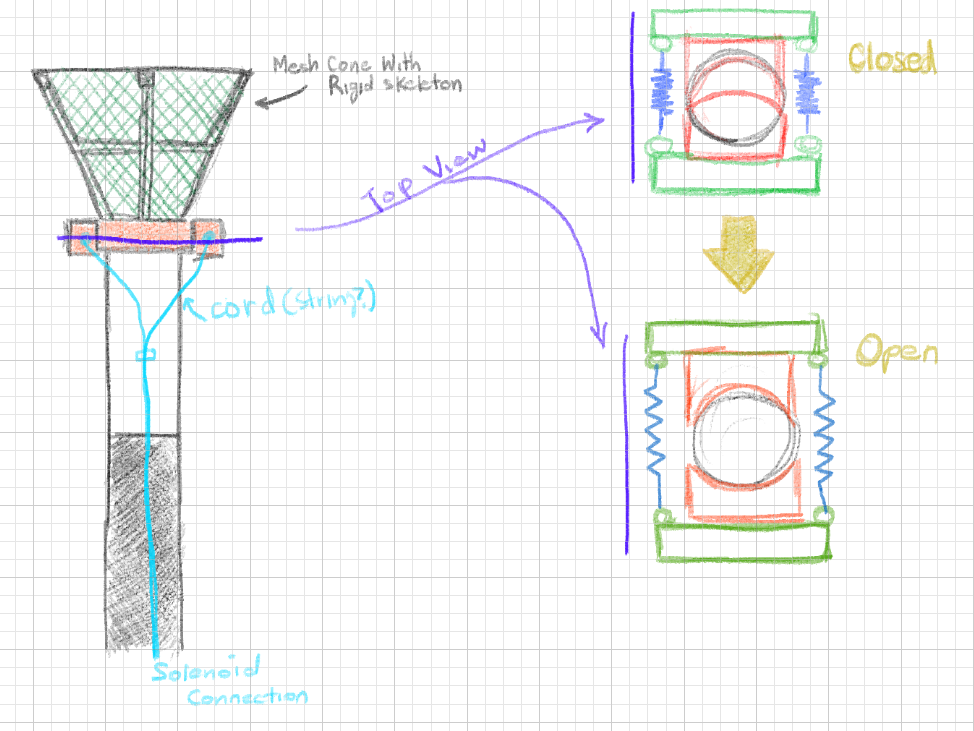
\includegraphics[width=\columnwidth]{figures/fig737.png}
\end{center}
\caption{Additional prototype sketch with solenoid concept included in cigar cutter}
\label{fig:7.3.7}
\end{figure}
\begin{figure}
\begin{center}
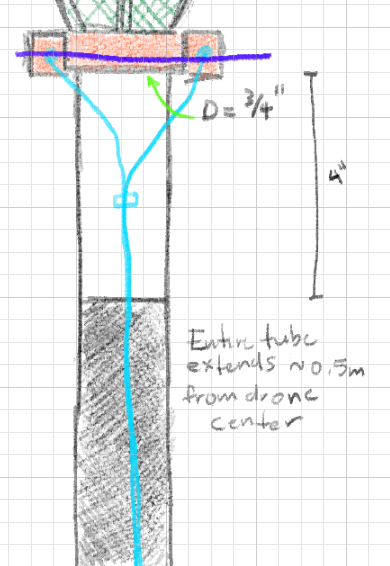
\includegraphics[width=0.49\columnwidth]{figures/fig738a.png}
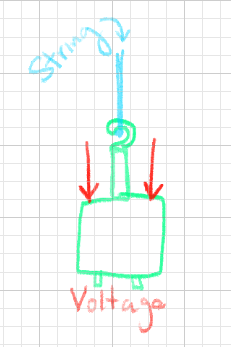
\includegraphics[width=0.49\columnwidth]{figures/fig738b.png}
\end{center}
\caption{More sketches of cigar cutter prototype with external power source for activation}
\label{fig:7.3.8}
\end{figure}
\begin{figure}
\begin{center}
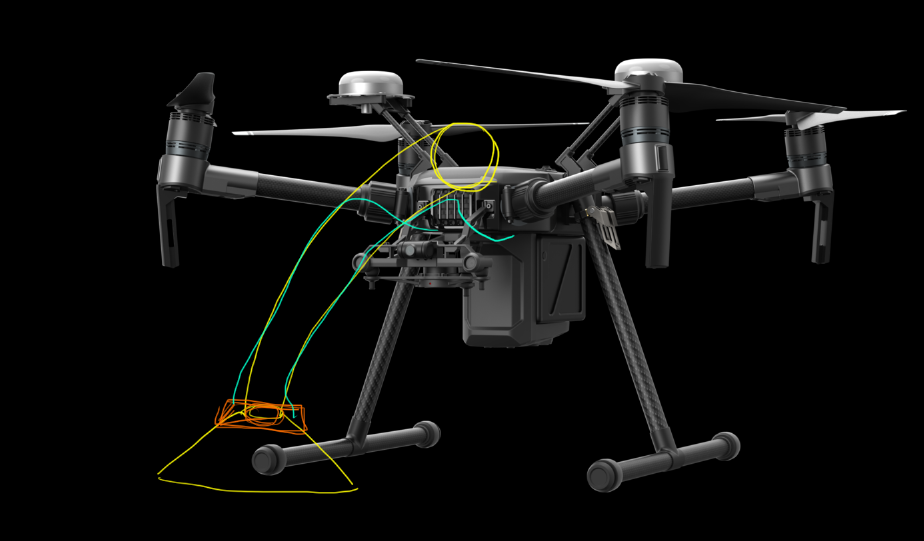
\includegraphics[width=\columnwidth]{figures/fig739.png}
\end{center}
\caption{Prototype sketch of final product prototyping}
\label{fig:7.3.9}
\end{figure}
\begin{figure}
\begin{center}
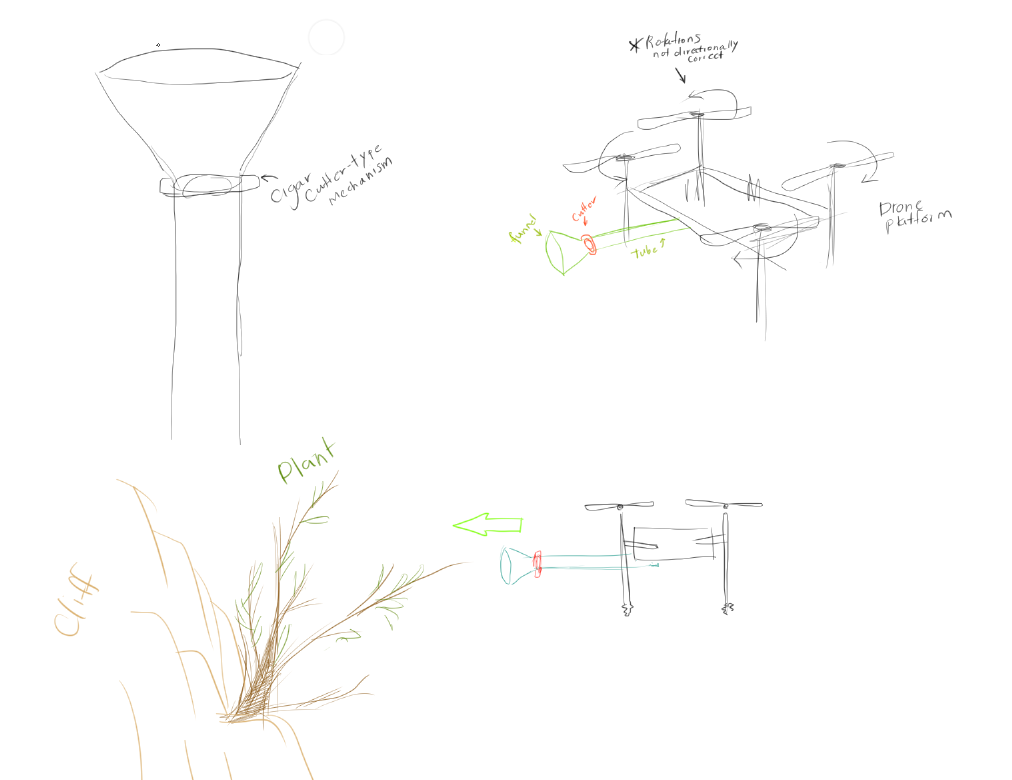
\includegraphics[width=0.8\columnwidth]{figures/fig7310.png}
\end{center}
\caption{Additional sketch of final product prototyping}
\label{fig:7.3.10}
\end{figure}
\begin{figure}
\begin{center}
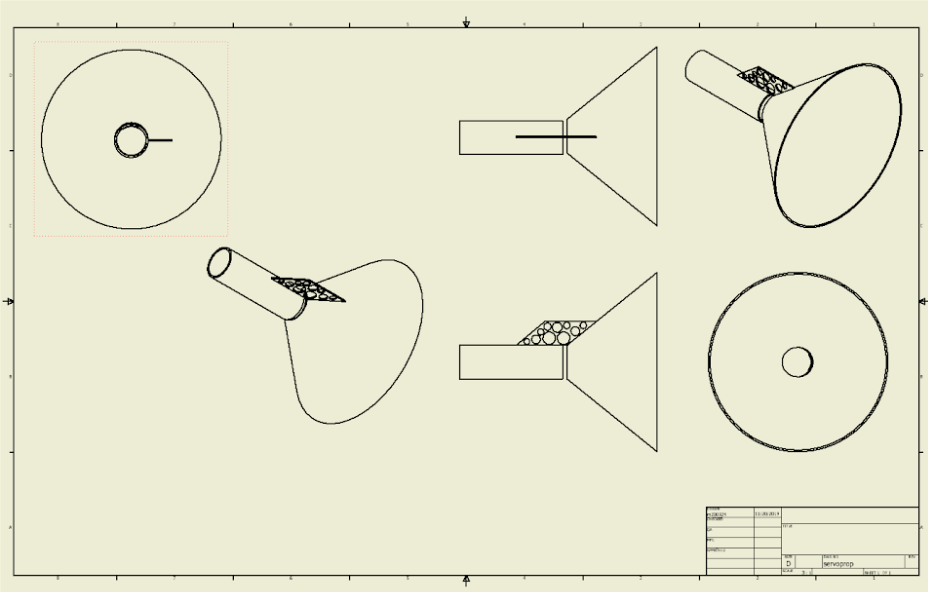
\includegraphics[width=\columnwidth]{figures/fig7311.png}
\end{center}
\caption{Digital prototype design for cone and tube if there were to be a servo attached.}
\label{fig:7.3.11}
\end{figure}





\subsection{Circuit Diagrams}
\begin{figure}
\begin{center}
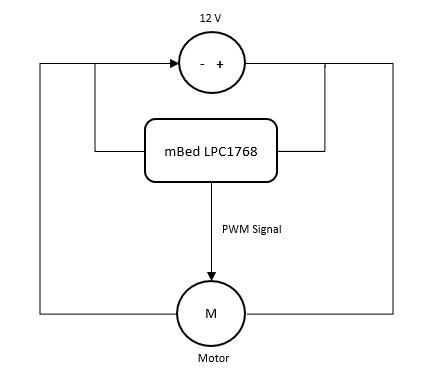
\includegraphics[width=0.6\columnwidth]{figures/fig741.png}
\end{center}
\caption{Basic Circuit Diagram of the Extraction Device}
\label{fig:7.4.1}
\end{figure}

\Fref{fig:7.4.1} shows the circuitry for the extraction device with a \SI{12}{\volt} power source, an LPC1768 microcontroller, and a motor. The LPC1768 has a recommended voltage input of \SIrange{4.5}{9}{\volt}, but it can function, with increased heat conversion, as long as the current is kept under \SI{150}{\milli\ampere}. as  We will use a \SI{12}{\volt} Motor to spin our end effector which is in parallel to the LPC 1768. The LPC 1768 will send a fixed PWM signal to the motor when prompted by the user.

This circuit represents the extraction device at a prototype level. In the air, the user will have to prompt the LPC1768 through wireless or radio communication. In the future, we will test with RC transmitters and receivers and incorporate them in the circuit to simulate a UAS in the air. 
\begin{figure}
\begin{center}
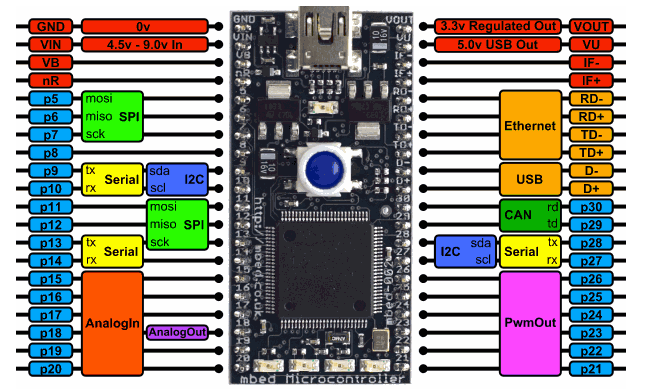
\includegraphics[width=\columnwidth]{figures/fig742.png}
\end{center}
\caption{Pin Allocations for the mbed LPC1768 Microcontroller \cite{mbed2019}}
\label{fig:7.4.2}
\end{figure}





\subsection{Prototypes}

\subsubsection{Parrot Bebop UAS}
\begin{figure}
\begin{center}
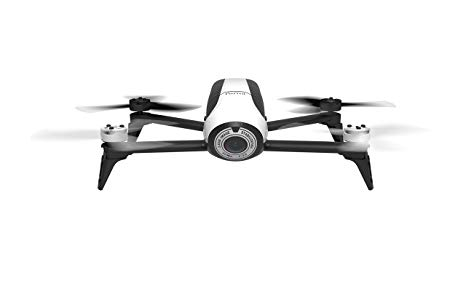
\includegraphics[width=0.3\columnwidth]{figures/fig751.png}
\end{center}
\caption{Parrot Bebop UAS \cite{parrot2019parrot}}
\label{fig:7.5.1}
\end{figure}
The Parrot Bebop UAS is a small scale prototype of the DJI Matrice 100. Testing on the prototype included video recording and putting a mock extraction device and see how it flew. This was before the DJI Matrice 100 was available for use. 

\subsubsection{Cigar Cutter Prototype}
\begin{figure}
\begin{center}
\includegraphics[height=1.3in]{figures/fig752a.png}
\includegraphics[height=1.3in]{figures/fig752b.png}
\includegraphics[height=1.3in]{figures/fig752c.png}
\end{center}
\caption{Cigar Cutter Prototype}
\label{fig:7.5.2}
\end{figure}
The cigar cutter prototype is fully functional and is able to accurately and reliably cut through stems. The plants are fed through the cigar cutter through a cone and are then cut using power from a set of springs.  Despite being a fully functional the design will need to be improved before it is ready to be mounted to the quadcopter.   

\subsubsection{Mouse Trap Prototype}
\begin{figure}
\begin{center}
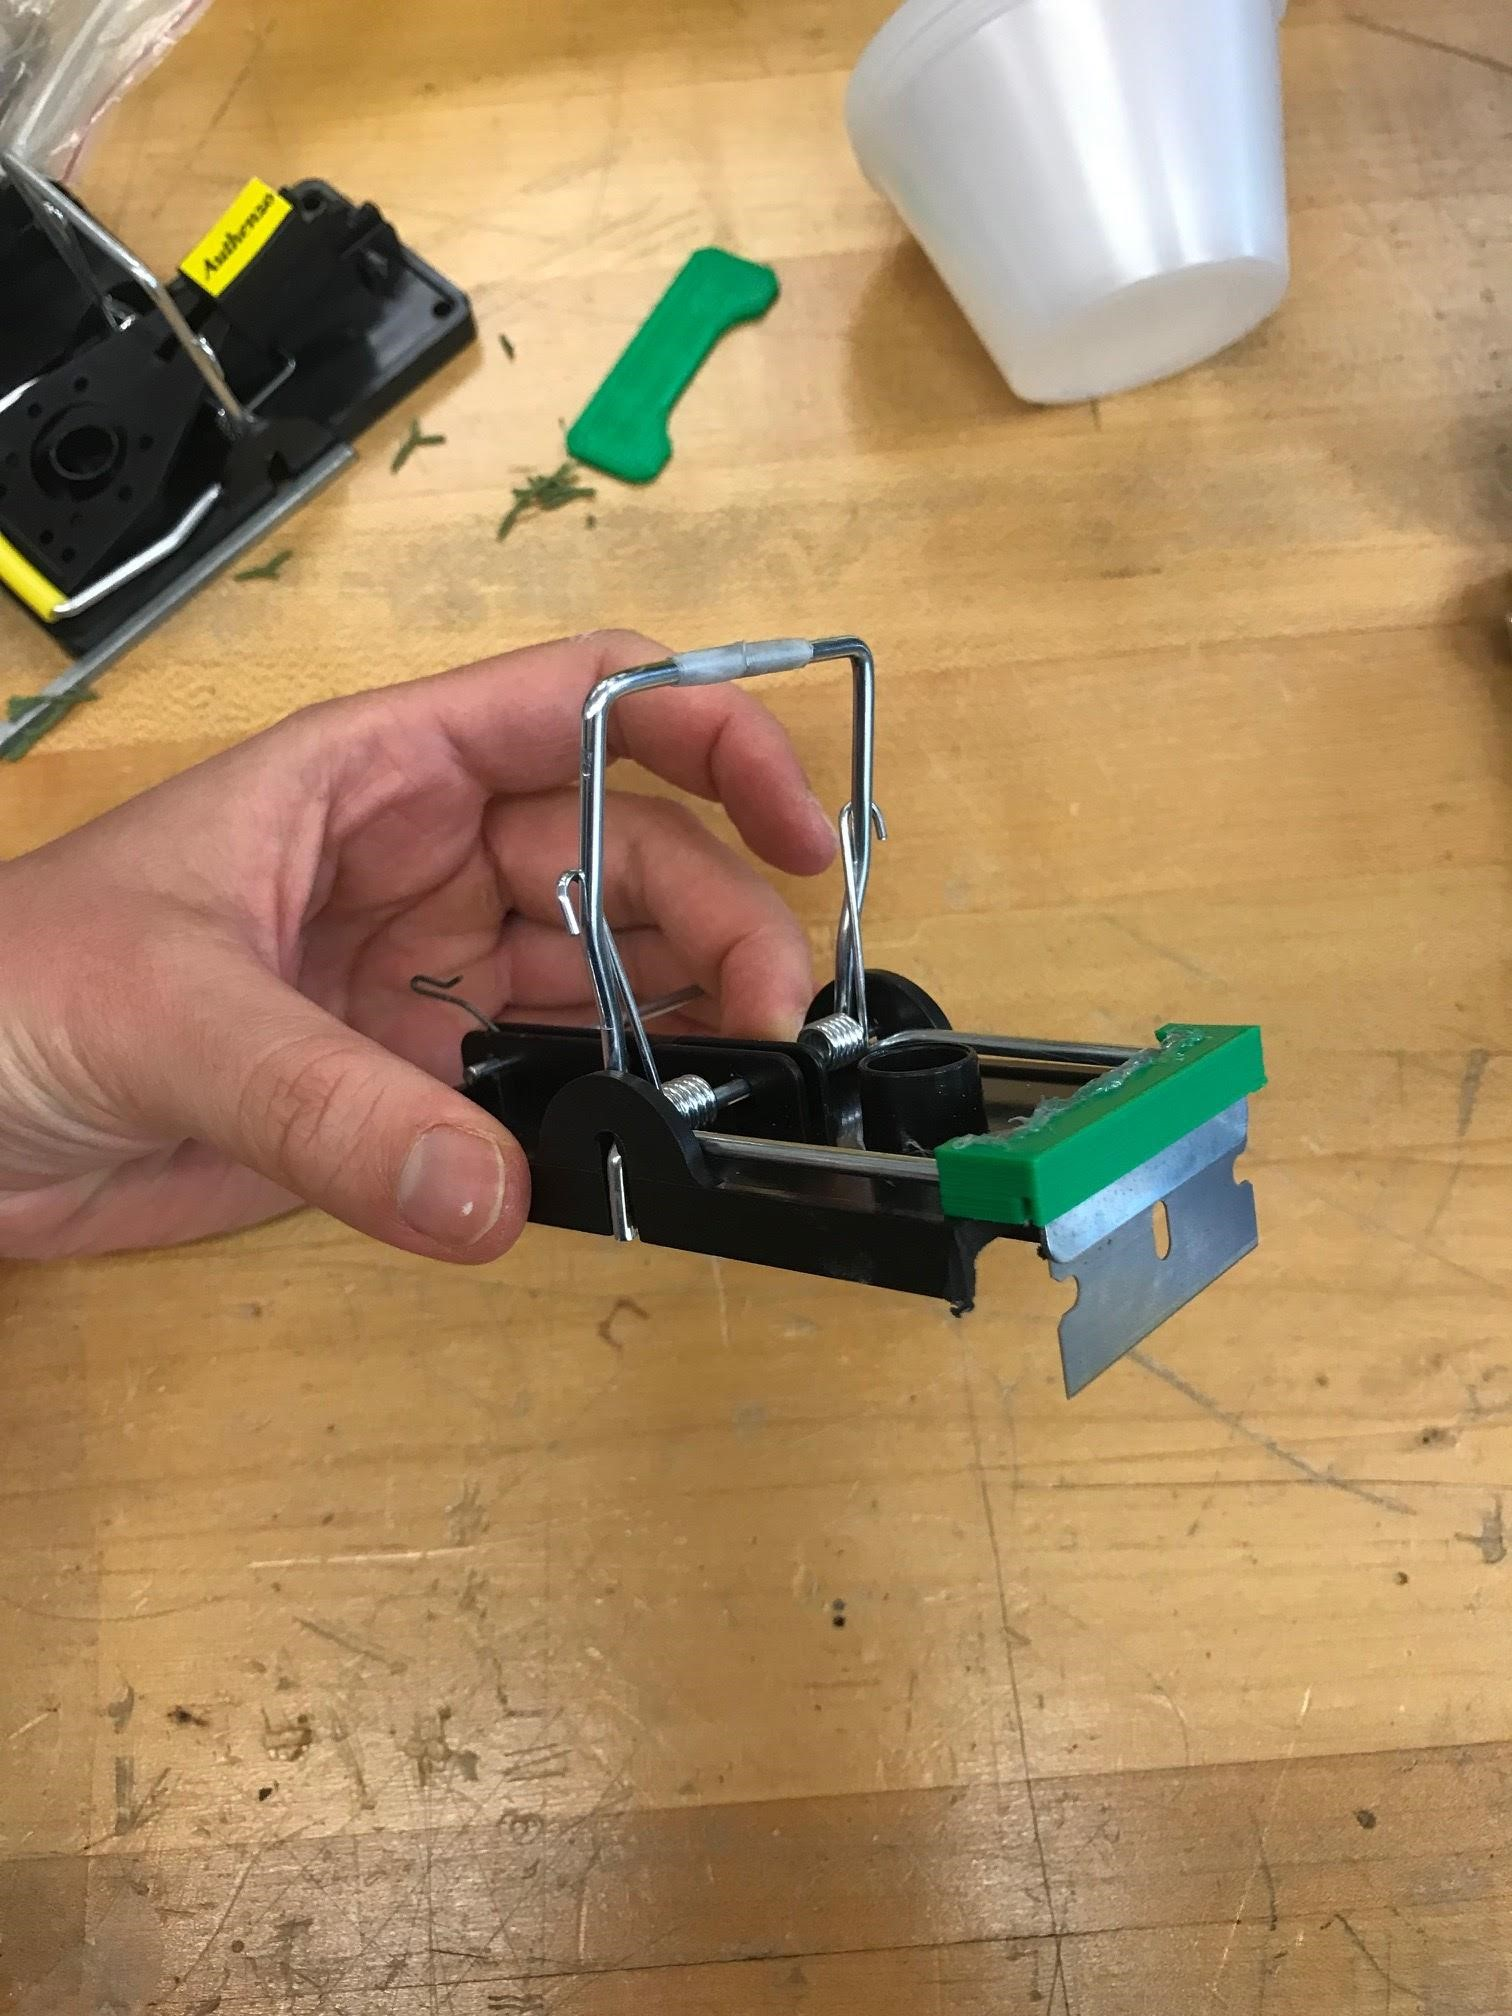
\includegraphics[width=0.5\columnwidth]{figures/fig753.jpg}
\end{center}
\caption{Mouse Trap Prototype}
\label{fig:7.5.3}
\end{figure}
The Mouse Trap Prototype is designed to cut through the plant with shear force as there is a blade attached to the mouse trap to ensure the plant is cut successfully. The mouse trap is positioned to the plant and when activated via a signal, the mouse trap prototype will close in on the plant snapping the sample from the main stem. 

\subsubsection{Mythbusters Motor Driven Shear and Servo Driven Gripper}
As seen in \fref{fig:7.5.4}, %??figure 4.5.1
the Motor Driven Sheer and Servo Driven Gripper are designed to more accurately cut and grip our desired plant. The motor drives a shaft connected to a worm drive. The worm drive will turn a gear that creates a linear motion through links that will moves the shears to open and close. Furthermore we will have a servo driven gripper placed on top of the shear to simultaneously grab onto the plant.
\begin{figure}
\begin{center}
\includegraphics[width=0.4\columnwidth]{figures/fig754a.png}
\includegraphics[width=0.4\columnwidth]{figures/fig754b.png}
\end{center}
\caption{Motorized Shear Prototype}
\label{fig:7.5.4}
\end{figure}





\subsection{Software Structure}
\begin{figure}
%\begin{center}
%\includegraphics[width=0.8\columnwidth]{figures/fig761.png}
%\end{center}
\lstinputlisting[style=mbedC]{code/mbed/motor-control/main.cpp}
\caption{Pseudocode for the mbed LPC1768 Microcontroller to Control a Motor}
\label{fig:7.6.1}
\end{figure}

The pseudocode in \fref{fig:7.6.1} shows the process of controlling a motor at the prompt of the user. The mbed continually sends PWM signals through a conditional while loop. When prompted by the user to start the motor, the mbed will send a higher PWM signal to the motor and change the variable which controls the while loop conditional. Another prompt will change the variable back to 0 which brings the code back to the original while loop.




\subsection{Simulations}

The simulations we conducted are more related towards how the operation would go if the group was in California. We simulated the test environment on Hospital Point with what was available to emulate the beginning of the UAS operation to the end. We measured out and taped the dimensions of the powered boat we would be on (\SI{20 x 6}{\foot}) and a ``landing platform'' on the side of the boat (\SI{6 x 6}{\foot}) where the UAS would take off and land from. 

In a Line of Sight Maneuver and live-stream received from the gimbal on the UAS, the UAS pilots (1/C Jisub Lim and 1/C Bryan) flew the UAS from the landing platform and tested out how the resolution was from the gimbal by flying close to the trees on Hospital Point. Afterwards, the UAS pilot conducted a landing maneuver onto the landing platform and timing how long it took to successfully land the UAS.

Other simulations/tests included battery life during flight maneuvers, testing the range of how far the UAS could go from the boat, and max speed tests as well. 

In regards to simulations for the extraction device, there are currently two prototypes that have been simulated. The mouse trap and cigar cutter extraction devices were manually held by hand. With a sample plant to test the extraction devices, the device was triggered by hand. We observed and recorded how the plant was cut. These are the simulations that have been conducted to emulate the subcomponents of the UAS and UAS operation. 







\section{Proposed Work}

\subsection{Work Breakdown Structure}
\begin{table}
\caption{Work Breakdown for each Team member}
\label{tab:8.1.1}
\begin{center}
\includegraphics[width=\columnwidth]{figures/table-811.jpg}
\end{center}
\end{table}

\subsection{Timeline}
\begin{table}
\caption{Timeline}
\label{tab:8.2.2}
\begin{center}
\includegraphics[width=0.8\columnwidth]{figures/table-821.png}
\end{center}
\end{table}

\clearpage
\begin{figure}
\begin{center}
%\includegraphics[angle=90,width=\columnwidth]{figures/table-822.png}
\includegraphics[width=\columnwidth]{figures/gantt.png}
\end{center}
\caption{Gantt Chart}
\label{tab:8.2.3}
\end{figure}





\subsection{Risk management}
\begin{table}
\caption{Risk of dropping UAS in water}
\label{tab:8.3.1a}
\includegraphics[width=\columnwidth]{figures/table-831a.jpg}
\end{table}

\begin{table}
\caption{Risk of not cutting plant completely}
\label{tab:8.3.1b}
\includegraphics[width=\columnwidth]{figures/table-831b.jpg}
\end{table}

\begin{table}
\caption{Risk of running out of battery / flight time}
\label{tab:8.3.1c}
\includegraphics[width=\columnwidth]{figures/table-831c.jpg}
\end{table}

\begin{table}
\caption{Risk of collision}
\label{tab:8.3.1d}
\includegraphics[width=\columnwidth]{figures/table-831d.jpg}
\end{table}

\begin{table}
\caption{Risk of crew overboard}
\label{tab:8.3.1e}
\includegraphics[width=\columnwidth]{figures/table-831e.jpg}
\end{table}

\begin{table}
\caption{Risk of actuation failure of snipper}
\label{tab:8.3.1f}
\includegraphics[width=\columnwidth]{figures/table-831f.jpg}
\end{table}

\begin{table}
\caption{Risk of getting lost at sea}
\label{tab:8.3.1g}
\includegraphics[width=\columnwidth]{figures/table-831g.jpg}
\end{table}

\begin{table}
\caption{Risk of injury while recovering UAS}
\label{tab:8.3.1i}
\includegraphics[width=\columnwidth]{figures/table-831i.jpg}
\end{table}









\subsection{Demonstration and Testing Plan}
For the UAS subsystem, we have tested what is possible to test for the UAS as of right now. We have recordings of the UAS taking and landing off through the tablet interface as well as one of us recording from the ground. The UAS battery life/operating time, max height and range, and the live-stream interface from the UAS have been observed and recorded during the test. We are devising a safe method to test the max payload capacity the UAS can hold since we are not able to attach the extraction device onto the UAS yet. With the recorded values of the tests conducted, they will be observed compared to the metrics and score it based on where it falls into the metrics.

For the extraction device, we will demonstrate the prototypes that we have made so far: the mousetrap, cigar cutter, and motorized shear extraction device prototypes. We will repeat the testing that’s been done on the three extraction devices with a sample plant to determine which one we will invest our resources into. The extraction device is configured into a circuit powered by an external battery/power source and controlled by an mbed microcontroller. Based on the metric parameters, such as the number of trials, the extraction device can be tested and we can observe the success rate of the different prototypes.








\section{Benchtop Demonstration}
\subsection{Activities}
During the final weeks of the semester, the extraction device team, Reina, Bryan and Levi, continued researching and designing for the extraction device prototypes, the three main designs being the mouse trap, motor driven snipper, servo driven gripper and cigar cutter devices. Jacob has a working circuit board that is available to test motors or servos connected to an extraction device to electrically power the extraction device. Jisub and Bryan are working on the UAS, getting flight time, and looking into other prototypes for the extraction device. We have also tested the live-stream from the UAS’s gimbal camera and marking certain distances and seeing how far the UAS can be while being able to identify a certain target which would be the plant. 
        
\subsection{Results}
\subsubsection{Operation simulation}
Test: Operation Simulation
Date: \printdate{11/21/2019}
Air Temperature: \SI{41}{\fahrenheit}
Experiment: The layout of the \SI{20x6}{\foot} power driven vessel was outlined in the grass of the field using masking tape. The boat that we will be training with has a maximum passenger capacity of 10. Our planned this test with seven passengers and the stern of the boat used for equipment. The passenger zone and the takeoff/landing zone was separated.  Available team members were positioned in the passenger section based on their role in UAS operations to test space availability during operations. Jacob is the boatswain, Ji is the pilot, Bryan is the Co-Pilot, Reina and Levi are note takers and safety observers. We made room for two other passengers on the boat. The goal of this test was to test safety during operations on a boat, space availability on the boat, and a full concept simulation of our operations.

Takeaways: 

During the operation simulation, we found that the DJI Matrice 100 UAS is very stable during flight and there were no issues with connection to the UAS at any range. Surveying the trees and surrounding environment showed positive results in which the quality of the camera was pretty good. We tested how close we could get to the trees and saw that the down drift on the UAS doesn’t affect the trees unless the UAS is directly above the tree. 

Landing maneuvers were conducted for both pilots (1/C Jisub and 1/C Bryan) and both landings were successful. We measured the distance from the center of the landing platform to the center of the drone. The data for that is discussed further below in the report. The space availability on the mock up of the boat was adequate, but there is a need for consideration of what type of boat we will be using in California as compared to the powered boat that is available at USNA. 
\begin{figure}
\begin{center}
\includegraphics[width=0.5\columnwidth]{figures/fig921.png}
\end{center}
\caption{A photo of the landing platform layout}
\label{fig:9.2.1}
\end{figure}
\begin{figure}
\begin{center}
\includegraphics[width=0.5\columnwidth]{figures/fig922.png}
\end{center}
\caption{A photo of the STEVE team simulating UAS operations from the boat}
\label{fig:9.2.2}
\end{figure}




\subsubsection{Battery life test}
Test: Battery Life
\begin{figure}
\begin{center}
\includegraphics[width=\columnwidth]{figures/fig923.png}
\end{center}
\caption{A graph showing the battery life of the TB48D (blue) and the TB47D (orange)}
\label{fig:9.2.3}
\end{figure}

The UAS was flown arbitrarily in increments of a few minutes in order to determine the actual battery life of the current UAS battery.  Each flight was a mixture of hovering and moving in order to familiarize the pilot (Jisub Lim) with the operation of the UAS.  The time and battery life after each flight was recorded.  The chart below shows the battery life against time for each test.  The blue line is the data for the flights done at small increments (\SIrange{2}{5}{\minute}) at a time using the TB48D battery, and the orange line shows the data for a longer flight made to deplete the battery completely (TB47D battery).

Takeaways:  

The battery life was shorter than the advertised battery due to varying conditions and likely due to wear. The battery may have been affected by the cold temperatures of the air. The UAS automatically lands when it hits 10\% battery life. The gimbal was not centered on the UAS platform, so there was always a slight offset when landing using only the camera




\subsubsection{Strength of twings}
Test: Strength of Twigs

Experiment: Using the purchased cigar cutter, twigs of different thicknesses will be tested in order to determine the relationship between the twig diameter and the force required to cut the twig.

In order to test how much force it takes to cut the branch, a scale was placed underneath the cigar cutter.  The blades were opened, the branch was fed into the hole, and the blades were pushed together by the scale on the bottom, and the hand on top.  The cedar branch was used because it is a fibrous plant that is harder to cut than most other plants.  Knowing the force required to cut each diameter can help us determine the amount of force our design needs to apply.  The test was conducted on two different plants: the cedar and the unknown softer twig.
\begin{table}
%\begin{center}
%\includegraphics[width=\columnwidth]{figures/table-921.png}
%\end{center}
\caption{Table testing required force to cut various twigs of various diameters}
\label{tab:9.2.1}
\begin{center}
\begin{tabular}{ccc}
\toprule
& twig diameter, \si{\milli\meter} & force to cut, \si{\poundforce} \\
\midrule
cedar & 4.9 & 34, 35, 38$_1$\\
cedar & 3.85 & 18 \\
cedar & 3.8 & 16 \\
cedar & 3.61 & 17 \\
cedar & 3.58 & 15 \\
cedar & 3.39 & 14 \\
cedar & 3.10 & 13 \\
softer & 1.66 & 0.31 \\
softer & 2.12 & 0.69 \\
softer & 2.4 & 0.81 \\
softer & 2.82 & 4 \\
softer & 3.06 & 9 \\
softer & 3.53 & 11, 11, 12$_1$\\
softer & 3.79 & 14 \\
softer & 3.75 & 14 \\
softer & 4.48 & 24 \\
softer & 4.56 & 24 \\
softer & 4.76 & 26 \\
\bottomrule
\end{tabular}
\vspace{2em}

$^1$multiple tests of same diameter
\end{center}
\end{table}


\begin{figure}
\begin{center}
\includegraphics[width=\columnwidth]{figures/fig924.png}
\end{center}
\caption{A graph showing the force required to cut vs the diameter of the branch}
\label{fig:9.2.4}
\end{figure}

Takeaways:
Branches are pretty hard to cut with a cigar cutter (sometimes the force required was close to \SI{40}{\poundforce}). There is some space between the blades that may cause slim, long, and flexible plants to deflect and not be cut fully. Clearly, the force increased with diameter, but the relationship was not linear

Imperfections of the experiment: The experiment only tests the twigs available to us in Annapolis.  The twigs that we will be taking samples from will probably have a slightly different composition because they are of a different species.  This test hopefully will give us a good idea on how strong the spring system must be in order to cut almost any potential sample.



\subsubsection{Time and difficulty of landing}
  
Test: Time and Difficulty of Landing

Experiment:
Two UAS pilots practiced landing the UAS in the allotted \SI{6x6}{\foot} box. The time it took to land the UAS after flying was recorded for each flight. The landing maneuver was defined as when the pilot concentrates solely on getting back on the platform after flying the UAS back to the boat.
After landing, the distance of the center of the UAS from the center of the platform was recorded in order to determine the offset caused by the location of the gimbal.  This bench test was also used in order to determine the best/most accurate UAS pilot for the experiment.

\begin{table}
\caption{Landing time and distance from platform center measurement for each UAS pilot}
\label{tab:9.2.2}
\begin{center}
\begin{tabular}{lll}
\toprule
landing time, \si{\second} & distance from platform center & UAS pilot \\
\midrule
48 & 8 & Ji \\
70 & 8 & Ji \\
90 & 12 & Bryan \\
95 & 15 & Bryan \\
\bottomrule
\end{tabular}
\end{center}
\end{table}
 
Takeaways: 
Jisub performed better as the UAS pilot than Bryan. The UAS lands automatically with the return-to-home feature which will not be applicable when the boat is moving. Angling the camera at \ang{90} is an accurate way to land manually. The other team members on the boat can assist with the landing of the drone as well. The UAS lands automatically at 10\% battery regardless of location, but there are a series of alarms and notifications before this happens.

\section*{Spring 2020 progress during the global COVID-19 pandemic}
In the Spring of 2020, as the global COVID-19 pandemic emerged, it became clear that the team's planned field mission to the California Channel Islands was not possible. Furthermore, with the Academy ordered to shift to remote instruction, there was no way to perform a local demonstration of the various stages of the original mission. As a result, the team decided to revisit several aspects from their concept and preliminary design reviews, and opted instead to take another trip around the design spiral, to improve the design further, for the benefit of future teams that attempt a field mission. Additional consideration was given to:
\begin{enumerate}
\item Further consideration of fixed wing and hybrid concepts to provide longer endurance during the survey phase of the mission (B.~Phan, \fref{sec:fixedwing})
\item Further consideration of machine vision aspects of the survey phase (J.~Kang, \fref{sec:vision})
\item Alternative quadrotor platforms to the DJI Matrice 100, due to DOD restrictions on DJI products (J.~Lim, \fref{sec:alternativequads})
\item Improvements to Matrice 100 hovering performance through additional sensors and control (J.~Lim, \fref{sec:hoveringcontrol})
\item Improved robot arm mechanical design (R.~Carroll and L.~Hofland, \fref{sec:robotarmmechanical})
\item Improved robot arm control design (J.~Kang, R.~Carroll and L.~Hofland, \fref{sec:robotarm})
\item Development of detailed operating and casualty procedures (J.~Kang, B.~Phan, and J.~Lim, appendices~\ref{app:OP} and \ref{app:CP})
\end{enumerate}

\subsection*{How STEVE could be used in response to COVID-19}
With the need for finding effective methods to mitigate COVID-19 pandemic spreading, there are several solutions that drones can offer during the crisis. Because STEVE is a platform that is aimed at carrying an extraction device capable of retrieving and securing plant samples from the origin and back, STEVE could serve public safety agencies in several aspects of the COVID-19 mitigation mission. By modifying the end effector and payload capacity, STEVE could retrieve and deliver medical supplies or testing kits to hard to reach places where hospitals or testing sites may not be readily accessible. STEVE could also return to the same destination to pick up the testing samples and return them to hospitals or testing sites for testing so that public safety employees don’t have to risk encountering those who may be affected by COVID-19. Furthermore, with computer vision, STEVE has the potential to monitor public spaces and identify large groups gathering and alert public safety agencies so that gatherings can be separated quickly. With agencies that already specialize in drone operations, STEVE could be quickly implemented for use without any large learning curve associated with it besides the end effector of the extraction device which could be modified for different missions in countering COVID-19.









\section{Further consideration of fixed wing and hybrid concepts to provide longer endurance during the survey phase of the mission (B.~Phan)}
\label{sec:fixedwing}

After initial flying experiences, it became clear that while the rotorcraft (e.g. quadrotors like DJI Matrice 100 or DJI Mavic Pro Platinum) could take off from a RHIB, fly towards the island, and film, they are limited in range due to the high power cost of hovering flight. Thus, we surveyed additional platforms further, considering fixed wing platforms (which would require arresting gear or similar recovery system), as well as hybrid VTOL platforms envisaged to be launched from the RHIB, fly mostly in an efficient fixed wing configuration, but be capable of vertical recovery onboard. 

\subsection{Rotorcraft}
\begin{figure}
\begin{center}
\includegraphics[width=0.49\columnwidth]{figures/survey1.png}
\end{center}
\caption{DJI Matrice 100 (baseline)}
\end{figure}

Platforms discussed: DJI Matrice 100

Platform tested: DJI Matrice 100

Attachments: (DJI Matrice 100) Zenmuse x3 camera, gimbal, TB47D battery, TB48D Battery

Objectives: This platform was our baseline. We wanted to find other systems that had greater endurance, camera quality and maneuverability when landing.

What tests were conducted: Battery life test with the TB87D and TD87D. Camera quality test while in flight. Gimbal maneuverability test. Line of Sight controllability. Reliability with the ground control station.

Landing Procedures Test: Landing operations on a \SI{6x6}{\foot} plank through line of sight (with help from safety observers), internal camera and combination of both.

Lessons Learned: At best with payload of the Zenmuse x3 camera and gimbal the battery would last for about \SI{15}{\minute}. Camera quality while live streaming was ok, when extracted for review it was spotty and glitchy. Gimbal could not yaw, and didn't really have an effect on the mission though because we were still able to angle to our desired locations. Landing was successful but took approximately 1 minutes from the drone being situated directly overhead the boat. Combination of LOS and FPV was best when used to land. FPV was adequate to fly when LOS was not an option. When the remote controller recognized Matice to have critical low battery it would automatically land wherever it was.
 
Recommendations for next year: After testing other systems, the Matrice 100 would not be a good choice for the survey aspect of the mission. Limited endurance and challenges with recovery would give $\sim\SI{10}{\minute}$ of flight time. Furthermore once the ground control station recognized the critical battery the system would auto land. Given a majority of the survey aspect is over water the operators would have to follow the Matrice around the island to mitigate risk of losing the system. Currently we only have 1 on hand. Furthermore given that each battery is $\sim$\$250 it would have been incredibly expensive to constantly change out.

\subsection{Fixed wing}
\begin{figure}
\begin{center}
\includegraphics[width=0.49\columnwidth]{figures/survey2a.png}
\includegraphics[width=0.49\columnwidth]{figures/survey2b.png}
\end{center}
\caption{Theory Type W. TBS Caipirinha 2}
\end{figure}

Platform: E-Flite Theory Type W, TBS Caipirinha 2

Platform tested: E-Flite Theory Type W

Attachments: (E-Flite Theory Type W) Stock with 4S \SI{1300}{\milli\ampere\hour} Lithium Batteries 

Objectives: Find a system when compared to the Matrice 100 would have longer endurance, better camera quality, autopilot and waypoint capabilities and recoverable from a RHIB.

What tests were conducted: (E-Flite Theory Type W) Practice flying to familiarize myself with the piloting procedures of a fixed wing aircraft. Was buddy-cabled and under the supervision of a licensed UAS trainer with this system for about two flight hours. Practiced different flight modes, launch, intermediate and experienced. Determined proficiency with total amount of hours practiced from someone who had zero experience)

Landing procedure tests: Goal post \SI{10}{\foot} apart with ``net''. Did not test wires and bouncy house methods. 

Lessons Learned: (E-Flite Theory Type W) This specific platform would not be used for the survey aspect of our mission and was tested solely to build proficiency. Starting from zero experience to about two flight hours I would categorize myself as still a beginner. I mainly operated the system in intermediate flight mode. Control of this platform was line of sight in all flights, we did not set up a first person view. After about two hours flight time I am comfortable taking off and doing basic movements such as figure eights and box patterns. However whenever the system was in an uncontrolled state, I did not have the ability to recover and needed to pass control to the UAS trainer. Further when landing the system through the goal post, I was successful 1/10 times collectively from multiple flights. The certified UAS trainer was successful 3/5 times from the same flight. The UAS trainer did this in intermediate mode and recommended this mode for future flights. The goal post was \SI{10}{\foot} apart and \SI{5}{\foot} high on stationary ground. 

(TBS Caipirinha 2) This system was not ordered or live tested in any capacity. However the advertised specifications were promising and worth looking into. The TBS Caipirinha 2 has about \SIrange{45}{90}{\minute} flight time, pre-cut FPV camera, battery, R/C receiver and video transmitter slots. Given the cost for a plug and play version is \$250.

Recommendations for next year: Given that a certified UAS Trainer was only successful recovering the system 3/5 times, I would only recommend this platform to a capable operator with flight experience. The dimensions of the goal post net will be much smaller on the RHIB with the added challenge of not being stationary. (TBS Caipirinha 2) Predicted challenges with this system are: it does not have an autopilot/waypoint function built in, the pre-cut camera slot affords users first person view but we predict that our flight pattern will be the perimeter of the island, meaning the angles would be off and a secondary camera must be installed.







\subsection{Seaplane}
\begin{figure}
\begin{center}
\includegraphics[width=0.49\columnwidth]{figures/survey4a.png}
\includegraphics[width=0.49\columnwidth]{figures/survey4b.png}
\end{center}
\caption{Avios Bushmule Seaplane; E-Flite Timber with floats (simulated)}
\end{figure}

Platform: Avios Bushmule (w/o float attachments), E-Flite Timber (with and without float attachment)

Platform tested: Avios Bushmule  (w/o float attachments), E-Flite Timber (simulated in RealFlight 9 program)

Objectives: Find a system when compared to the Matrice 100 would have longer endurance, better camera quality, autopilot and waypoint capabilities and recoverable by a RHIB.

What tests were conducted: (Avios Bushmule) Practice flying to familiarize myself with the piloting procedures of a fixed wing aircraft. Was buddy-cabled and under the supervision of a licensed UAS trainer with this system for about two flight hours. Practiced different flight modes, beginner, intermediate and advanced. Determined proficiency with total amount of hours practiced from someone who had zero experience. Tested my ability to land. Tested the flight time of the system. All tests were conducted line of sight

(E-Flite Timber without float attachments) Practiced flying to gain experience similarly to previous platforms, however used the RealFlight 9 simulation system to complete ``challenges'' that reflected necessary skills for the survey mission. The challenges built into the simulation were called spot landing and air race. Spot landing graded the accuracy a user was able to land on a desired point. Air race practices maneuverability and precision by passing through an array of gates. All tests were conducted line of sight. I did not find an option to access FPV while in ``challenge mode''

(E-Flite Timber with float attachments) Practiced the take off and landing dynamics of a seaplane in water. While in a simulated environment, I wanted to test the differences in technique of land based landing and water based. Test consisted of a mixture of FPV and line of sight.

Landing procedure tests: Avios Bushmule (w/o float attachments) and E-Flite Timber (without float attachment) Tested spot landing at a predetermined area \SI{10x10}{\foot}.

E-Flite Timber (with float attachment) Practice ability to land in water, noted different techniques and dynamics that water based landing required. Attempted to repeatedly land at the same spot.  
Lessons Learned: The Avios Bushmule  (w/o float attachments) was an easier/forgiving plane to pilot. Because it moves slower, I was able to recover from piloting mistakes. With a single battery we were able to get about \SI{15}{\minute} fight time. The system offers additional payload but that was not tested. Discovered landing was relatively similar to other fixed wing platforms.

(E-Flite Timber with and without float attachments) I have about \SI{5}{\hour} flight time in the simulated environment with this type aircraft. I took the lessons covering fundamentals of flight and tried the challenges offered. Even after \SI{5}{\hour} flight time I would categorize myself as a beginner pilot. Flying line of sight is extremely challenging for me. After making piloting mistakes, I would usually be unable to recover. I was only able to reach level 2 on each of the challenges. When landing the (E-Flite Timber with float attachments) the operator must pitch the aircraft upwards slightly and reduce speed on approach. If the aircraft isn't pitch and going too fast, it will nosedive into the water. Furthermore, when the aircraft lands the underbelly gets wet.  

Recommendations for next year: The ability to land airplanes on water is extremely promising, however further research needs to be done regarding the sea state of the landing areas. The lack of endurance of the models we conclude further research needs to be done for longer duration systems. There is a high probability for the system to get wet so waterproofing the camera system may be necessary. 



\subsection{Fixed wing tail sitter VTOL}
\begin{figure}
\begin{center}
\includegraphics[width=0.49\columnwidth]{figures/survey3a.png}
\includegraphics[width=0.49\columnwidth]{figures/survey3b.png}
\end{center}
\caption{E-Flite X-Vert; FireFly 6 Pro}
\end{figure}

Platform: E-Flite X-Vert, FireFLY 6 Pro

Platform tested: E-Flite X-Vert

Attachments: (E-Flite X-Vert) Stock with \SI{800}{\milli\ampere\hour} Lithium Batteries

Objectives: Find a system when compared to the Matrice 100 would have longer endurance, better camera quality, autopilot and waypoint capabilities and recoverable from a RHIB.

What test were conducted: (E-Flite X-Vert) Practice flying to familiarize myself with the piloting procedures of a fixed wing VTOL aircraft. Practiced different flight modes, multirotor, stability and ACRO. Determined proficiency with total amount of hours practiced from someone who had zero experience.

Landing procedure tests: (E-Flite X-Vert) Tested the ability to land in \SI{5x5}{\foot} box both indoor and outdoor. Tested the ability for a person to catch the UAS midair. Tested how the system reacted when held (simulated caught from landing) on full throttle. 

Lessons Learned: The X-Vert is too small to use for the actual mission. It was extremely sensitive to even light windy conditions ($\geq\SI{5}{\mph}$). When in multirotor mode and full throttle the system routinely was unable to fight the strength of the wind and would have to make an emergency landing. These landing were nowhere near the original \SI{5x5}{\foot} box. When in stability mode the system responded better to windy conditions but was still difficult to operate. Noteworthy, when the system was too hard to control, switching back to multirotor mode acted as a failsafe to give inexperienced operators (myself) the ability to hover and regain control.  Indoor tests were successful and we were able to perform touch and gos, ang{360} yaw rotations, and translational movements within the box. Furthermore, Dr. Evangelista (wearing PPE) caught the X-Vert mid-air followed by motor disarm. When Dr. Evangelista held the X-Vert while I attempted to drive it up at full throttle, the system was easily controllable.  I found that the VTOL capabilities were extremely useful in the takeoff and landing aspect of the survey mission. Given a bigger platform this system looks very promising.

(FireFLY 6 Pro) This system has not been tested in any capacity but multiple recently have been ordered by the Weapons department. The advertised specifications prominent to the survey aspect of our mission are; approximately \SI{50}{\minute} flight time from takeoff to landing, can carry a payload of at least \SI{1.25}{\pound}, AvA (Advanced VTOL Autonomy) software that runs on the PX4hawk (aka Pixhawk) autopilot. 

\subsection{Recommendation: VTOL}

Given my inexperience as a UAS operator, I feel the most comfortable piloting VTOL systems. The ability to land like a rotorcraft exponentially lowers the learning curve for newer pilots. Throughout all systems tested I have researched/tested, the FireFLY 6 Pro is the most promising. An expected challenge is that the small area for takeoff and landing is \SI{10x10}{\foot} which is larger than the RHIB we will operate in. 


\subsection{Recommendation: Use of simulators, and early training}

Simulator flights should be the first mastered before attempting to live fly aircraft. I broke both the theory type W and the X-Vert from my inexperience operating a fixed wing system. I have approximately \SI{5}{\hour} of simulated flight time and approximately \SI{2}{\hour} of live flight time and still categorize myself as a beginner. Whenever the system was in an uncontrolled state, I did not have the ability to recover.  I am comfortable taking off and doing basic movements such as figure-eights and box patterns. However when landing strictly fixed wing systems I do not have the capability to accurately pilot the systems through a goal post \SI{10x10}{\foot} wide on a stationary ground. Furthermore, I do not have the capability to land a fixed wing with and without floats repeatedly on a \SI{10x10}{\foot} plot. I do have the capability using VTOL to land on a \SI{6x6}{\foot} stationary plot. Given the volatile nature of the mission having a competent driver is necessary meaning if you want to be the pilot you need to put the hours in! 

If given the chance I would be most confident in piloting the FireFLY 6 Pro. 
       
%
%
%        f you do, write down what you learned and how the procedure changed after trying it in sim - that's important because it's important to know why the steps in a procedure are the way they are
%
%
% and then give metrics of how successful you are at it after n days of training so that future-Phan-wannabes have an idea how long it might take to train for the mission.
%
%
%What did he learn from test flights, 
%develop selection matrix, 
%more detailed preliminary design, etc. If there is an arresting system to be designed, work with MEs to design it; if there is a tail sitter concept, identify type (WingTraOne, stolen from Blount design, etc), same for seaplane. What payload is to be flown, what is its autopilot and which Pixhawk does it need. PArt ordering info, weight and cost estimate if possible.
%
%
%Phan: Concept and preliminary design for the Survey Mission, considering 
%
%
%What did he learn from test flights, develop selection matrix, more detailed preliminary design, etc. If there is an arresting system to be designed, work with MEs to design it; if there is a tail sitter concept, identify type (WingTraOne, stolen from Blount design, etc), same for seaplane. What payload is to be flown, what is its autopilot and which Pixhawk does it need. PArt ordering info, weight and cost estimate if possible.
%  
%e. Somewhere in there I think Lim (maybe with help from Phan) was going to look for a scalign tool or something tog ive first order estimation of range, speed, endurance, payload vs airframe vs battery weight and relationships between these. If you can find a scaling tool and learn how to use it great; if it requires generating some basic scalings via Mathcad (NAOEtype) or Matlab or whatever that works too.
\section{Further consideration of machine vision aspects of the survey phase (J.~Kang)}
\label{sec:vision}

The purpose of this section is to discuss plant identification and image stitching, two necessary machine vision applications that would increase the chances of the survey mission successfully locating specimens of interest for retrieval. 

\subsection{Plant Identification}
Plant Identification is identifying plants with the survey drone using premade software. This was a low priority element of our CAPSTONE, but the research was important in case future groups wanted to implement it into their design. 

\subsection{Softwares and Methods}
\begin{itemize}
\item PlantId
\begin{itemize}
\item Free software 
\item Requires an upload of five plants weekly to maintain subscription
\item Seems to only work on image uploads and some plants may require multiple images of the same plant for proper identification
\item Would be difficult to implement into our system.
\end{itemize}
\item Convolutional Neural Networks
\begin{itemize}
\item This is basically deep learning for computer imaging. To a computer, an image is just a large matrix of RGB values, and it is possible to train a computer to recognize these RGB values and create a probability of what the image is about.
\item The process begins with neurons and weight. Each neuron can be thought of as a feature filter and uses small pixel sections of the entire image to determine what feature that pixel section represents.
\item Each pixel section uses its filter to output a number and these new numbers now can be used to determine higher level features, they now act as neurons going through a new filter. This can be visualized as a neural network. 
\item This process must be trained by using many different images. Each time the CNN is trained it alters the weights of its filter choices in order to improve its classification. This training process is what makes a CNN considered a deep learning algorithm. 
\item Further details of CNNs can be found in this link \url{https://adeshpande3.github.io/A-Beginner\%27s-Guide-To-Understanding-Convolutional-Neural-Networks/}
\end{itemize}
\item iNaturalist
\begin{itemize}
\item This software is similar to PlantId, but it is used for all animal life.
\item The identification does not come from code but from crowdsourcing done by experts in order to identify a specimen.
\item Images or Video taken from the survey drone can be uploaded to the iNaturalist website and await results from experts there.
\end{itemize}
\end{itemize}
\begin{figure}
\begin{center}
\includegraphics[width=\columnwidth]{figures/vision1.png}
\end{center}
\caption{Image taken from \url{https://adeshpande3.github.io/A-Beginner\%27s-Guide-To-Understanding-Convolutional-Neural-Networks/} to explain convolutional neural networks (CNNs).}
\end{figure}

\subsection{Image Stitching}
The vision for image stitching is to use images taken by the survey drone to recreate a map of the survey area. 


The following images and code were taken from \Matlab\ to provide an example on panoramic image stitching. In this folder contain two codes: \lstinline{ImageStitch.m}, my code (appendix~\ref{app:C2}), and \lstinline{FeatureBasedPanoramicImageStitching.m} (appendix~\ref{app:C1}), code taken from \Matlab. \lstinline{ImageStitch} is code I created in order to replicate \Matlab’s code for testing my own images taken from my room. After hours spent trying to fix it, there are still some problems that I cannot figure out. The problem seems to stem from the image format and pixel size, and I cannot figure out why the images are rotated \ang{90} when imported into \Matlab.

Figures~\ref{fig:vision1} and \ref{fig:vision2} show the result of running \Matlab’s code using their source images. It works extremely well and figuring out image formatting and more time with this code can mean creating image stitched maps of our own for the survey mission.
  
\begin{figure}
\begin{center}
\includegraphics[width=0.8\columnwidth]{figures/vision2.png}
\end{center}
\caption{Five Images of a Building}
\label{fig:vision1}
\end{figure}
  
\begin{figure}
\begin{center}
\includegraphics[width=\columnwidth]{figures/vision3.png}
\end{center}
\caption{The Images Connected through Feature Based Panoramic Image Stitching}
\label{fig:vision2}
\end{figure}
\section{Alternative quadrotor platforms to the DJI Matrice 100, due to DOD restrictions on DJI products (J.~Lim)}
\label{sec:alternativequads}

With the main problems of the DJI Matrice 100 being the fragile balance between payload and ample flight time, it is recommended that an alternative is a drone that is capable to flying up to \SI{45}{\minute} or more with payload attached to the drone. The following platforms that are larger than the DJI Matrice 100 are listed below:
\begin{enumerate}
\item \textbf{DJI Matrice 210 RTK V2.} The Matrice 210 RTK V2 is a new model that DJI has released but is still not out in the market currently. It is a quadcopter that operates with two TB55 batteries. The max payload the drone can carry is \SI{1.34}{\kilo\gram} ($\sim\SI{3}{\pound}$). Although the battery life is longer than the DJI matrice 100, it is still relatively short with a max flight time of \SI{24}{\minute} with max payload and \SI{34}{\minute} without payload. The drone has an ultrasonic sensor for hovering accuracy that operates from \SIrange{0.33}{16.4}{\foot}. 

\item \textbf{DJI Matrice 600 Pro.} The DJI Matrice 600 Pro is a six propeller drone that is widely used as the platform for large scale missions such as farming lands. With six TB48S batteries, the Matrice 600 is capable of flying with a \SI{5.5}{\kilo\gram} payload for \SI{18}{\minute} and can fly without a payload for \SI{38}{\minute}.
\end{enumerate}

Unfortunately, both identified platforms are DJI projects which will soon be subject to more extensive DOD bans and are not being recommended for future USNA procurement. 
\section{Improvements to Matrice 100 hovering performance through additional sensors and control (J.~Lim)}
\label{sec:hoveringcontrol}

The DJI Matrice 100 equipment had an attachable guidance system which has optic flow ultrasound sensors. This guidance system has the main central unit along with the frame surrounding it so that the four usable sensors can be adjusted in position for whichever direction you want to avoid colliding in. We worked on configuring the drone setup if it was to fly with the guidance system along and still have space to attach the extraction arm and end effect. The configuration was valid, however, there were some issues that arose after configuring the drone. The guidance system must be powered from the drone by using the XT60 power adapter cord, however, the length of the XT60 power cord was not long enough to reach the power outlet that connects to the drone and the power inlet for the guidance system. 

As seen in the pictures, one sensor was attached below the drone while the other three sensors were attached to the main frame of the guidance system up top. The reason for this configuration was because during the sample recovery mission, the drone needs to stay stable when hovering. The guidance system is able to detect velocity between \SIrange{0}{16}{\meter\per\second} and has an accuracy of \SI{0.04}{\meter\per\second} velocity detection (\SI{2}{\meter} above the ground). The sensors’ effective range is between \SIrange{0.20}{20}{\meter}. Because the effective range is up to \SI{65}{\foot}. The bottom sensor can track how the drone is moving based on what’s below the drone whether it is a sloped ground or the ocean next to the cliff. 

The guidance system can prove to be very helpful in the mission because stability of the drone during the sample recovery mission was one of the main issues the mission was difficult. If the drone is able to stabilize at an altitude high enough where there sensors are still effective, the drone may be stable enough where the drone pilot doesn’t have to worry about stabilizing the drone when hovering in close proximity of the plant. This also has the potential to change the way the extraction device is designed in which the extraction device might not need to be countering the drone’s movement while hovering, but rather just able to focus on grabbing the plant and securing the plant sample. 

\begin{figure}
\begin{center}
\includegraphics[width=\columnwidth]{figures/hovering1.png}
\end{center}
\caption{Specifications of the guidance system}
\label{fig:hovering1}
\end{figure}

\begin{figure}
\begin{center}
\includegraphics[width=\columnwidth]{figures/hovering2.png}
\end{center}
\caption{DJI Matrice 100 with guidance system attached on top}
\label{fig:hovering2}
\end{figure}

\begin{figure}
\begin{center}
\includegraphics[width=0.8\columnwidth]{figures/hovering3.png}
\end{center}
\caption{Back view of DJI Matrice with Guidance System}
\label{fig:hovering3}
\end{figure}

\begin{figure}
\begin{center}
\includegraphics[width=0.8\columnwidth]{figures/hovering4.png}
\end{center}
\caption{Bottom View of Matrice 100 with bottom sensor attached}
\label{fig:hovering4}
\end{figure}

\begin{figure}
\begin{center}
\includegraphics[width=0.8\columnwidth]{figures/hovering5.png}
\end{center}
\caption{XT60 power adapter cord needed to power guidance system. Cord length must be longer.}
\label{fig:hovering5}
\end{figure}

\section{Improved robot arm mechanical design (L.~Hofland and R.~Carroll}
\label{sec:robotarmmechanical}

The preliminary design concept did not have a well accepted robot arm / snipper / gripper concept for taking and retaining the sample. As a result, in Spring 2020, the team brainstormed and developed futher concepts for the robot arm / snipper / gripper and backed them up with prototype testing, including a ``lawnmower'' (propeller snoot chopper), a ``guillotine'' nonchopping snoot, a pip3 arm, and a buzzsaw concept. The buzzsaw concept was recommended for further development. 

\begin{enumerate}
\item Telescoping razor blades:
\begin{figure}
\begin{center}
\includegraphics[height=1.5in]{figures/robotarmmech1a.png}
\includegraphics[height=1.5in]{figures/robotarmmech1b.png}
\end{center}
\end{figure}
\begin{enumerate}
\item Pros: snips and grips with one fluid motion
\item Cons: complex, hard to build
\item Primary failure: unreliable cut and likely blade failure
\item Design Rejected
\end{enumerate}

\item Bladed jaw
\begin{figure}
\begin{center}
\includegraphics[height=1.5in]{figures/robotarmmech2a.png}
\includegraphics[height=1.5in]{figures/robotarmmech2b.png}
\end{center}
\end{figure}
\begin{enumerate}
\item Pros: simplified design
\item Primary failure: unable to cut catastrophic blade failure during testing.
\item Design Rejected
\item Notes: design powered by a mousetrap
\end{enumerate} 

\item Automated Pruning shears
\begin{figure}
\begin{center}
\includegraphics[height=1.5in]{figures/robotarmmech3.png}
\end{center}
\end{figure}
\begin{enumerate}
\item Pros: verified cutting capability under ideal conditions
\item Cons: complex, heavy
\item Primary failure: Gipping design difficult
\item Design Rejected
\end{enumerate}

\item Cigar Cutter
\begin{figure}
\begin{center}
\includegraphics[height=1.5in]{figures/robotarmmech4a.png}
\includegraphics[height=1.5in]{figures/robotarmmech4b.png}
\includegraphics[height=1.5in]{figures/robotarmmech4c.png}
\end{center}
\end{figure}
\begin{enumerate} 
\item Pros: successful test of both snipping and gripping. Simple design, easily operated, lightweight
\item Primary failure: One shot one kill
\item Design Rejected
\end{enumerate}

\item Propeller snoot chopper
\begin{enumerate}
\item Pros: controllable, simple, lightweight, snipping and gripping take place simultaneously.   
\item Primary failure: Sample is blended; for botanical voucher specimen use, intact leaves, fruits, and flowers are desired. Blended samples also risk mixing DNA. 
\item Design Rejected
\end{enumerate}

\item Nonchopping snoot
\begin{figure}
\begin{center}
\includegraphics[height=1.5in]{figures/robotarmmech6.png}
\end{center}
\end{figure}
\begin{enumerate}
\item Pros: Sample is not blended
\item Primary failure: After testing this design failed to snip even a small branch
\item Design Rejected
\end{enumerate}

\item Pipe Arm
\begin{figure}
\begin{center}
\includegraphics[height=1.5in]{figures/robotarmmech7.png}
\end{center}
\end{figure}
\begin{enumerate}
\item Lightweight, functional, balanced
\item Primary failure: design rejected in favor of controllable robotic arm. 
\end{enumerate}

\item Buzzsaw arm grabber
\begin{figure}
\begin{center}
\includegraphics[height=1.5in]{figures/robotarmmech8.png}
\end{center}
\end{figure}
\begin{enumerate}
\item Pros: Controllable, lightweight, captures samples in one piece
\item Mounted on the end of a robotic arm. 
\item The cutting blade attached to a propeller engine
\item Lightweight netting is strung between the``fingers'' of each ``hand'' to capture the sample.
\item Current snipper/gripper design 
\end{enumerate}
\end{enumerate}

\section{Improved robot arm control design (J. Kang, L.~Hofland, and R.~Carroll)}
\label{sec:robotarm}

This section describes an improved robotic arm and control scheme for the DJI Matrice 100.

\subsection{Introduction}
The Biomechanics team tested different solutions on which apparatus would be best for reaching the plant. We finalized that the best solution would be a joint controlled robotic arm controlled by an mbed that communicates with the user through telemetry communication. This document will discuss the thought process in building the robotic arm. It will not discuss the gripper component.

\subsection{Background and Controls}
The goal of the project is to use a drone to cut and retrieve plant material. Our group set a condition that all plants would be cut when the drone is landed. The plants desired by Dr. Guilliams were generally low to the ground and landing the drone before cutting would reduce the risk of losing control of the drone. 

The Robot Arm will be controlled by an Mbed LPC1768 that is connected to the user for control through telemetry. There will be separate batteries that amount to a total of \SI{6}{\volt} for powering both the Mbed and the Servos in the Robot Arm. Example code is given in appendix~\ref{app:D}

\subsection{Parts Used}
\begin{enumerate}
\item 1xMbed LPC1768
\item 3xServos (\ang{90}-\ang{180} RoM)
\item Robot Building Pieces (Can be found in the EW202 Classroom) or can be 3D printed to be lighter
\item Telemetry Equipment (RFD900 Long Range Telemetry) or Wireless Transceiver (nRF24L01) or Long Range Xbee
\item Small Camera (GoPro Hero Session)
\end{enumerate}

\subsection{Robot Workspace}
We built the robotic arm to be a RRR arm for maximum range of motion. This allows the drone pilot to land anywhere near the plant and the robot will still be able to reach the plant. An arm less than an RRR arm would potentially waste battery life if the drone needed to move reposition. 
\begin{itemize}
\item Joint 1: Allows for 90 degrees of motion in the X-Y Plane
\item Joint 2: Allows for 90 degrees of motion in the Y-Z Plane
\item Joint 3: Allows for 90 degrees of motion in the Y-Z Plane
\end{itemize}

\begin{figure}
\begin{center}
\includegraphics[width=0.8\columnwidth]{figures/robotarm1.png}
\end{center}
\caption{RRR Arm Model with all Joints at \ang{0}}
\label{fig:robotarm1}
\end{figure}

\begin{itemize}
\item Joint 1: Allows for 90 degrees of motion in the Y-Z Plane
\item Joint 2: Allows for 90 degrees of motion in the Y-Z Plane
\item Joint 3: Allows for 90 degrees of motion in the X-Y Plane
\end{itemize}

\begin{figure}
\begin{center}
\includegraphics[width=0.8\columnwidth]{figures/robotarm2.png}
\end{center}
\caption{RRR Arm in Alternate Position}
\label{fig:robotarm2}
\end{figure}

\subsection{Torque}
The Average torque for a servo running at \SI{6}{\volt} is \SI{0.988}{\newton\meter}. The plants we are working with will be light in weight and the arm will not have a problem with torque in carrying the plants. This was concluded through testing with the prototype arm we built. We used heavy metal pieces from the EW202 classroom and the arm still moved very well.

\begin{figure}
\begin{center}
\includegraphics[width=\columnwidth]{figures/robotarm3.png}
\end{center}
\caption{Mbed Pinout}
\label{fig:robotarm3}
\end{figure}

\subsection{Mbed Configuration}
The Mbed will be on top of the drone body frame. The pins used for servo control are \lstinline{p21}, \lstinline{p22}, and \lstinline{p23} for \lstinline{PwmOut}. Commands for the Mbed can be sent through Teraterm or a Matlab User Interface. 

\subsection{Camera}
There must be an additional camera placed near the base of the robot arm so the user can see what the arm is doing in real time. We were thinking of the GoPro Hero Session because of its small size and quality. 

\subsection{Biggest Challenges}
We have not done any testing on how telemetry will work between the User’s computer and the Mbed, so that is a problem we are still facing. Example code for Mbed telemetry can be found online and I added one in this folder. Another option if telemetry is deemed overkill is an Mbed specific wireless transceiver called the nRF24L01. It could be used for sending video data and commands from the user wirelessly, but it only has a range of \SI{100}{\meter}. Another option is and Xbee capable of long range wireless communication.

We need testing on if a \SI{6}{\volt} battery will be enough to power the Mbed and all three servos. 

We need testing on the best place to place the additional camera and how to connect it to the Mbed and then to the user.




\section*{Acknowledgements}
\addcontentsline{toc}{section}{Acknowledgements}
We thank Dr. Alison Webster-Giddings, Professor Devries, Professor Dawkins, Mrs Burgett, Mr Bradshaw, and Mr Rhodes for their assistance with all aspects of our project. We also thank Mason Fridge, Luke Knollinger, Delfino Garia, Lenny Davis, Kevin Lee, and Sean Kee for their advice regarding autonomous and radio controlled flight. We thank our customer, Dr. Matt Guilliams and the Santa Barbara Botanical Garden. We also thank Prof David Johnston and the Duke Marine Lab UAS group. The 2019 Biomechanics capstone team (ENS Edwards, Hall, Nemani, Martin), kindly helped us get started with a good turnover. The USNA biomechanics seminar also helped us understand the need for engineers in field ecology and biological studies. USNA Biomechanics is supported by Lockheed Martin. USNA School of Drones is supported by Broering and by Boeing. 

\nocite{hyneman2017jamie, famoussmoke2019cigar} % never used? 
%\section{References}
\addcontentsline{toc}{section}{References}
\bibliography{biosteve.bib}


% Appendices here (optional)
\clearpage
\appendix
\renewcommand{\figurename}{Supplementary Figure}
\renewcommand{\thefigure}{S\arabic{figure}}
\clearpage
\section{Operating procedures for Matrice 100 (J.~Lim)}
\label{app:OP}

\subsection{START OF DAY CHECKLIST}

\subsubsection{Firmware update}
\begin{enumerate}
\setlength{\itemsep}{0em}
\setlength{\parskip}{0em}
\item Ensure firmware is updated to the latest version
\end{enumerate}

\subsubsection{Battery charging}
\begin{enumerate}
\setlength{\itemsep}{0em}
\setlength{\parskip}{0em}
\item Ensure LiPo Battery are supervised at ALL times when charging
\item Look out for any puffing or inflating of battery in any state (charging or when stored)
\item Make sure tablet is fully charged and supervised when charging
\end{enumerate}

\subsubsection{Inventory Check}
\begin{enumerate}
\setlength{\itemsep}{0em}
\setlength{\parskip}{0em}
\item Make sure all all components of aircraft are in the aircraft case
\item Make sure extraction device is properly stored 
\end{enumerate}



\clearpage
\subsection{Go - No Go Checklist}
\textbf{Requirement to proceed: Must go through every item in above checklist}

\subsubsection{Weather}
Go: 
\begin{enumerate}
\setlength{\itemsep}{0em}
\setlength{\parskip}{0em}
\item Clear skies
\item Calm waters
\item Low precipitation
\item  Low wind speeds ($<\SI{22}{\meter\per\second}$)
\end{enumerate}

\textbf{No Go:}
\begin{enumerate}
\setlength{\itemsep}{0em}
\setlength{\parskip}{0em}
\item Any indication of rain, fog, thunderstorms
\item High wind speeds ($>\SI{22}{\meter\per\second}$)
\item Heavy waves
\end{enumerate}

\subsubsection{Equipment Status}
Go: 
\begin{enumerate}
\setlength{\itemsep}{0em}
\setlength{\parskip}{0em}
\item Frame- Check for no damage
\item Screw check- Ensure tightness (frame, standoffs, motors, camera)
\item Wire check- Ensure no damage (fraying, disconnections, etc)
\item Ensure gimbal is mounted correctly and tightly
\item Ensure extraction device is mounted correctly and tightly (when applicable)
\item Connection between tablet and aircraft are securely established
\end{enumerate}

\textbf{No Go:}
\begin{enumerate}
\setlength{\itemsep}{0em}
\setlength{\parskip}{0em}
\item Any damage found on frame 
\item Loose screws
\item Disconnected or exposed wires 
\item Gimbal not securely attached
\item Extraction device is loose and susceptible to hitting propellers
\item Unable to connect to aircraft through tablet
\item Lag or spotty response from remote controller or tablet
\end{enumerate}

\textbf{Requirement to proceed: Must go through every item in above checklist}







\clearpage
\subsection{DJI MATRICE 100 PREFLIGHT CHECKLIST}
\textbf{Note: GPS Mode assumed}

\subsubsection{Walk Around}
\begin{enumerate}
\setlength{\itemsep}{0em}
\setlength{\parskip}{0em}
\item Frame- Check for damage
\item Screw check- Ensure tightness (frame, standoffs, motors, camera)
\item Wire check- Ensure no damage (fraying, disconnections, etc)
\item Ensure gimbal is mounted correctly and tightly
\item Ensure extraction device is mounted correctly and tightly (when applicable)
\end{enumerate}

\subsubsection{Before Start}
\begin{enumerate}
\setlength{\itemsep}{0em}
\setlength{\parskip}{0em}
\item Verify all batteries are full
\begin{enumerate}
\setlength{\itemsep}{0em}
\setlength{\parskip}{0em}
\item Verified by pressing power button once
\item Full battery status if, all four bars are lit 
\item If all lights are lit, charge battery if possible
\end{enumerate}
\item Select battery and attach (\textbf{Do NOT connect to JST})
\item Attach propellers. \textbf{Ensure correct rotation}, screw check
\begin{figure}[h]
\begin{center}
\includegraphics[width=0.4\columnwidth]{figures/op1.png}
\end{center}
\end{figure}  
\item Attach propeller guards onto aircraft
\item Ensure remote controller is on with sticks centered
\end{enumerate}

\subsubsection{Starting}
\begin{enumerate}
\setlength{\itemsep}{0em}
\setlength{\parskip}{0em}
\item Communicate that you will be powering on; Deconflict if needed
\item Connect battery to battery compartment
\item Power on for battery by pressing power button once and then pressing power button until all bars are lit
\item IMMEDIATELY place on flat surface
\item Connect tablet to remote controller via cable
\item Connect tablet to aircraft via wifi
\item Verify video feed on RS Go app, verify gimbal full range of motion and quality of video feed
\item Establish that Front LEDs, Rear LEDs, and Aircraft Status Indicator are working and lights are indicating that the aircraft is operable:
\begin{figure}[h]
\begin{center}
\includegraphics[width=0.8\columnwidth]{figures/op2.png}
\end{center}
\end{figure}  
\begin{figure}[h]
\begin{center}
\includegraphics[width=0.6\columnwidth]{figures/op3.png}
\end{center}
\end{figure}  
\item \textbf{DO NOT PROCEED IF WARNING LIGHTS ARE FLASHING}
\item Refer to Aircraft Status Indicator Description chart and resolve issues if applicable. If unresolvable do not operate Matrice until error/warning is resolved. 
\item Ensure extraction device is powered on and operable (when applicable)
\item Prop areas- clear 
\end{enumerate}



\clearpage
\subsubsection{Calibrating Compass Procedure}
\textbf{WARNING:}
\begin{enumerate}
\setlength{\itemsep}{0em}
\setlength{\parskip}{0em}
\item \textbf{DO NOT} Calibrate compass where there is a chance of strong magnetic interference, such as magnetite quarries, parking structures, and underground steel reinforcements
\item \textbf{DO NOT} carry ferromagnetic objects such as keys with you during calibration
\item \textbf{DO NOT} calibrate besides massive metal objects
\item \textbf{DO NOT} calibrate in an indoor space
\end{enumerate}

Proceed once pilot has read through warning section:
\begin{enumerate}
\setlength{\itemsep}{0em}
\setlength{\parskip}{0em}
\item Choose an open space to carry out the procedures
\item Ensure the compass is calibrated. If you did not calibrate the compass as part of your pre-flight preparations, or if you have moved to a new location since the last calibration, tap the System Status bar in the app and select Calibrate, then follow the on-screen instructions to calibrate the aircraft step-by-step
\item Hold the aircraft horizontally, and rotate it 360 degrees along the central axis. The Aircraft Status Indicator will emit a solid green light
\item Hold the aircraft vertically with its nose pointing downwards, and rotate it 360 degrees around its central axis 
\item Recalibrate the compass if the Aircraft Status Indicator becomes solid red
\item If the Aircraft Status Indicator flashes red and yellow alternatively after compass calibration, move your aircraft to a different location to carry out the calibration
\end{enumerate}

\textbf{ALWAYS RECALIBRATE if:}
\begin{enumerate}
\setlength{\itemsep}{0em}
\setlength{\parskip}{0em}
\item The compass data is abnormal, and the Aircraft Status Indicator is flashing red and yellow alternatively 
\item Flying in a new location, or a location that is different from your last flight
\item The mechanical structure of the Matrice 100 is changed, i.e. the mounting position of the GPS module is changed. 
\item Severe drifting occurs in flight, i.e. Matrice 100 has difficulty flying in a straight line. 
\begin{figure}[h]
\begin{center}
\includegraphics[width=\columnwidth]{figures/op4.png}
\end{center}
\caption{Calibrating compass procedure}
\end{figure}  
\end{enumerate}

  
\clearpage
\subsubsection{Motor Runup}
\begin{enumerate}
\setlength{\itemsep}{0em}
\setlength{\parskip}{0em}
\item Perform Combination Stick Command (CSC) to start/stop the motors. Ensure that you perform the CSC in one continuous motion
\begin{figure}[h]
\begin{center}
\includegraphics[width=0.7\columnwidth]{figures/op5.png}
\end{center}
\end{figure}  
\item Perform CSC Command. The motors will begin to speed at an idle speed, with the aircraft remaining stationary. 
\item With motors spinning, verify correct rotation
\item At idle, control test (``control surfaces'')- Pitch, roll, yaw
\item Throttle- test to verify response, but do not take off 
\item \textbf{TO STOP MOTORS:} There are two methods:
\begin{enumerate}
\setlength{\itemsep}{0em}
\setlength{\parskip}{0em}
\item Method 1: When the Matrice 100 has landed, push the throttle stick stick down, then perform the CSC command to stop the motors. Release both sticks once the motors have stopped
\item Method 2: When the aircraft has landed, push the throttle down and hold. The motors will stop after a few seconds. 
\end{enumerate}
\begin{figure}[h]
\begin{center}
\includegraphics[width=\columnwidth]{figures/op5.png}
\end{center}
\end{figure}   
\item \textbf{DO NOT} perform the CSC command when the aircraft is in mid-air. 
\end{enumerate}

\subsubsection{Before Takeoff}
\begin{enumerate}
\setlength{\itemsep}{0em}
\setlength{\parskip}{0em}
\item Clear- ensure takeoff area is clear
\item Talk- verbally alert other pilots that you are taking off, and state immediate intentions
\end{enumerate}


\clearpage
\subsubsection{Takeoff/Landing Procedures}
\textbf{WARNING:}
\begin{enumerate}
\setlength{\itemsep}{0em}
\setlength{\parskip}{0em}
\item When the Aircraft Status Indicator flashes yellow rapidly during flight, the aircraft has entered Failsafe mode
\item The Aircraft Status Indicator will flash red slowly for a Low Battery Level Warning, and flash red rapidly for a Critically Low Battery Level Warning during flight
\item \textbf{AIRCRAFT WILL LAND AUTOMATICALLY WHEREVER IT IS WHEN REACHING CRITICALLY LOW BATTERY LEVEL WARNING DURING FLIGHT}
\item Recover Aircraft back to home point \textbf{IMMEDIATELY} when Return to Home Status or Low Battery Level Warning is indicated on mobile device or tablet
\item Do not use aircraft in adverse weather conditions including raining, snowing, fog, and wind speeds exceeding (\SI{10}{\meter\per\second})
\item Only fly in open areas. Tall buildings and steel structures may affect accuracy of the compass and the GPS signal
\item Avoid flying near obstacles, crowds, high voltage power lines, trees and bodies of water. 
\item Avoid flying in area with high levels of electromagnetism
\item Aircraft and battery performance is subject to environmental factors such as air density and temperature
\item Matrice 100 cannot operate in P-Mode within the Earth’s polar region

\textbf{IN THE EVENT PILOT HAS LOST GPS SIGNAL AND CAMERA SIGNAL:}
\begin{enumerate}
\setlength{\itemsep}{0em}
\setlength{\parskip}{0em}
\item Alert all personnel that pilot has lost aircraft signal
\item If aircraft is in Field of View and has auto landed at current location, pinpoint and record location for aircraft recovery if recoverable
\item If aircraft is in Field of View and is still operable by remote controller, maneuver aircraft towards the home point \textbf{IMMEDIATELY}
\item \textbf{PROCEED TO RECOVERY PROCEDURE}
\end{enumerate}

Proceed once pilot has read and is aware of above warning section:
\item If applicable, place the aircraft on an open, flat ground with the battery indicator facing you
\item Power on the remote controller and your mobile device, then the Intelligent Flight Battery
\item Launch the DJI GO or RS GO app and enter Camera View
\item Wait until the Aircraft Status Indicator flashes green. This means the Home Point is recorded and is safe to fly. If it flashes yellow, the Home Point has not been recorded and you should not take off
\item Push the throttle stick up slowly to take of or use Auto Takeoff
\item Too land, hover over a level surface and gently pull down on the throttle stick to descend slowly
\item After landing, execute the CSC command or push the throttle stick down for 3 seconds until the motors come to a stop
\item Turn off the Intelligent Flight Battery followed by the remote controller
\end{enumerate}


 
\subsubsection{Recovery Procedure for Boat Operation (if applicable)}
\textbf{WARNING: IN THE EVENT OF CASUALTY DURING RECOVERY PROCEDURE, FOLLOW CASUALTY PROCEDURE IMMEDIATELY. DO NOT PROCEED RECOVERY PROCEDURE}
\begin{enumerate}
\setlength{\itemsep}{0em}
\setlength{\parskip}{0em}
\item Ensure that recovery personnel are strapped with protection gear and standing by at the landing region for recovery. \textbf{DO NOT} proceed if recovery personnel are not ready.
\item Ensure desired landing region is clear of any debris and the person recovering is secured and has given verbal communication to begin recovery
\item Maneuver aircraft so that aircraft is right above landing platform 
\item Adjust gimbal so that camera view is directly on top of recovering personnel and make verbal communication that camera view is centered on landing personnel
\item Announce that you are landing the aircraft to personnel
\item Ensure that personnel are always keeping an eye on the aircraft and must give verbal feedback on aircraft positioning while landing
\item Slowly lower throttle and lower aircraft unless otherwise instructed by recovery personnel
\item Once recovery personnel has secure grip of the aircraft and has given verbal communication that aircraft is secured, \textbf{IMMEDIATELY} perform CSC command to stop motors
\begin{figure}[h]
\begin{center}
\includegraphics[width=\columnwidth]{figures/op6.png}
\end{center}
\end{figure}  
\item Turn off Flight Battery and remote controller
\end{enumerate}



\clearpage
\subsection{DJI Matrice 100 Post-flight checklist}
\textbf{Note: GPS Mode assumed}

\subsubsection{Walk Around}
\begin{enumerate}
\setlength{\itemsep}{0em}
\setlength{\parskip}{0em}
\item Frame- Check for damage 
\item Screw check- Ensure tightness (frame, standoffs, motors, camera)
\item Wire check- Ensure no damage (fraying, disconnections, etc)
\item Ensure gimbal is not damaged and still operating
\item Ensure extraction device is intact and secured
\item Make sure battery is still working and at operable temperature
\end{enumerate}

\subsubsection{Securing the sample}
\begin{enumerate}
\setlength{\itemsep}{0em}
\setlength{\parskip}{0em}
\item Make sure there is no sharp protruding parts from the extraction device
\item Carefully unlatch sample vessel containing the sample
\item Confirm if sample is the right sample collected and of sufficient size
\end{enumerate}

\subsubsection{In the event of more flights}
\begin{enumerate}
\setlength{\itemsep}{0em}
\setlength{\parskip}{0em}
\item Go through DJI Matrice 100 Pre-flight checklist
\item Ensure extraction device is reset and ready
\item Ensure fully charged battery is used at operable temperature
\end{enumerate}

\subsubsection{Disassembly}
\begin{enumerate}
\setlength{\itemsep}{0em}
\setlength{\parskip}{0em}
\item Ensure the DJI Matrice, controller, and tablet are all turned off
\item Take off propellers and prop guards 
\item Unscrew extraction device from aircraft
\item Unscrew gimbal mount and camera
\item Secure the aircraft components into case
\end{enumerate}
\clearpage
\section{Boat operation and drone casualty procedures (J.~Kang, B.~Phan, and J.~Lim)}
\label{app:CP}

\subsection{Safety Measures}
\begin{enumerate}
\setlength{\itemsep}{0em}
\setlength{\parskip}{0em}
\item No Leaning over the boat. 
\item No Limbs outside of the boat. 
\item Wear PFD at all times.
\end{enumerate}


\subsection{Crew Overboard (owner: Kang)}
\begin{enumerate}
\setlength{\itemsep}{0em}
\setlength{\parskip}{0em}
\item Locate the crew overboard and approach slowly. 
\item When getting closer to the victim, shift engines to neutral and keep the propellers away from the victim. 
\item Stop and turn off the engines and proceed to make contact with the individual. 
\item Check the person for injuries and throw a personal floatation device to the person in the water.
\end{enumerate}


\subsection{Drone in the water (owner: Kang)}
\begin{enumerate}
\setlength{\itemsep}{0em}
\setlength{\parskip}{0em}
\item Locate drone and approach expeditiously in case the drone sinks. 
\item When getting closer, shift engines to neutral and grab the drone out of the water. 
\item Another member must hold the shirt of anyone performing a task requiring a member to reach outside the boat to prevent man overboards.
\end{enumerate}


\subsection{Abandon ship (owner: Kang)}
Loss of Engine, Control. Call Channel Islands National Park: (805) 658-5730. Contact USCG: VHF-FM Channel 16 (\SI{156.8}{\mega\hertz}), dial 911 (There is a USCG Unit in Santa Barbara). In the case of no cell signal, use paddles on boats to go towards the large islands where there is cell service. Confirm what boat we are using and if they provide paddles.


\subsection{Loss of telemetry (owner: Kang)}
A loss of telemetry on the Extraction Drone will make us unable to complete the extractino mission. Immediately return Drone to ship and recharge batteries while Kang, Ji, and Lim work on troubleshooting the telemetry. Telemetry will be done through an Mbed and all three members have experience with that microcontroller.


\subsection{Loss of FPV (Phan, Lim)}

\textbf{IN THE EVENT PILOT HAS LOST GPS SIGNAL AND CAMERA SIGNAL:}
\begin{enumerate}
\setlength{\itemsep}{0em}
\setlength{\parskip}{0em}
\item Alert all personnel that pilot has lost aircraft signal
\item If aircraft is in Field of View and has auto landed at current location, pinpoint and record location for aircraft recovery if recoverable
\item If aircraft is in Field of View and is still operable by remote controller, maneuver aircraft towards the home point \textbf{IMMEDIATELY}
\item \textbf{PROCEED TO RECOVERY PROCEDURE}
\end{enumerate}


\subsection{Loss of drone control (Phan, Lim)}

\textbf{IN THE EVENT PILOT HAS LOST GPS SIGNAL AND CAMERA SIGNAL:}
\begin{enumerate}
\setlength{\itemsep}{0em}
\setlength{\parskip}{0em}
\item Alert all personnel that pilot has lost aircraft signal
\item If aircraft is in Field of View and has auto landed at current location, pinpoint and record location for aircraft recovery if recoverable
\item If aircraft is in Field of View and is still operable by remote controller, maneuver aircraft towards the home point \textbf{IMMEDIATELY}
\item \textbf{PROCEED TO RECOVERY PROCEDURE}
\end{enumerate}


\subsection{Drone crash on deck or land (owner: Phan, Lim)}


\subsection{Battery fire (owner: Phan, Lim)}
Class D fire, needs a specific estingisher to put out. Reccomended from XXX authority is to XXX.


\subsection{Additional Information}
There is \textbf{no public WiFi} available at this time on the islands or at the mainland visitor center in Ventura. Cell service is available on the mainland including at the visitor center in Ventura. On the islands, \textbf{cell service is spotty and should not be relied upon}. This means most of the time visitors to the islands will not have cell service. In an emergency, locate park or concessioner staff.

\url{https://www.nps.gov/chis/planyourvisit/basicinfo.htm}

\clearpage
\section{\Matlab\ code}
\label{app:C}

\subsection{\lstinline{FeatureBasedPanoramicImageStitchingExample.m}}\label{app:C1}
\lstinputlisting[style=usnaMatlab]{code/matlab/FeatureBasedPanoramicImageStitchingExample.m}

\subsection{\lstinline{ImageStitch.m}}\label{app:C2}
\lstinputlisting[style=usnaMatlab]{code/matlab/ImageStitch.m}
\clearpage
\section{mbed robot arm control code}
\label{app:D}

\lstinputlisting[style=mbedC]{code/mbed/robot-arm-control/main.cpp}

\end{document}